
\section{Getting to know Klimahuset}
\par
\emph{26.01.2021, initial contact and visiting Klimahuset for the first time}
\par

\begin{figure}[H]
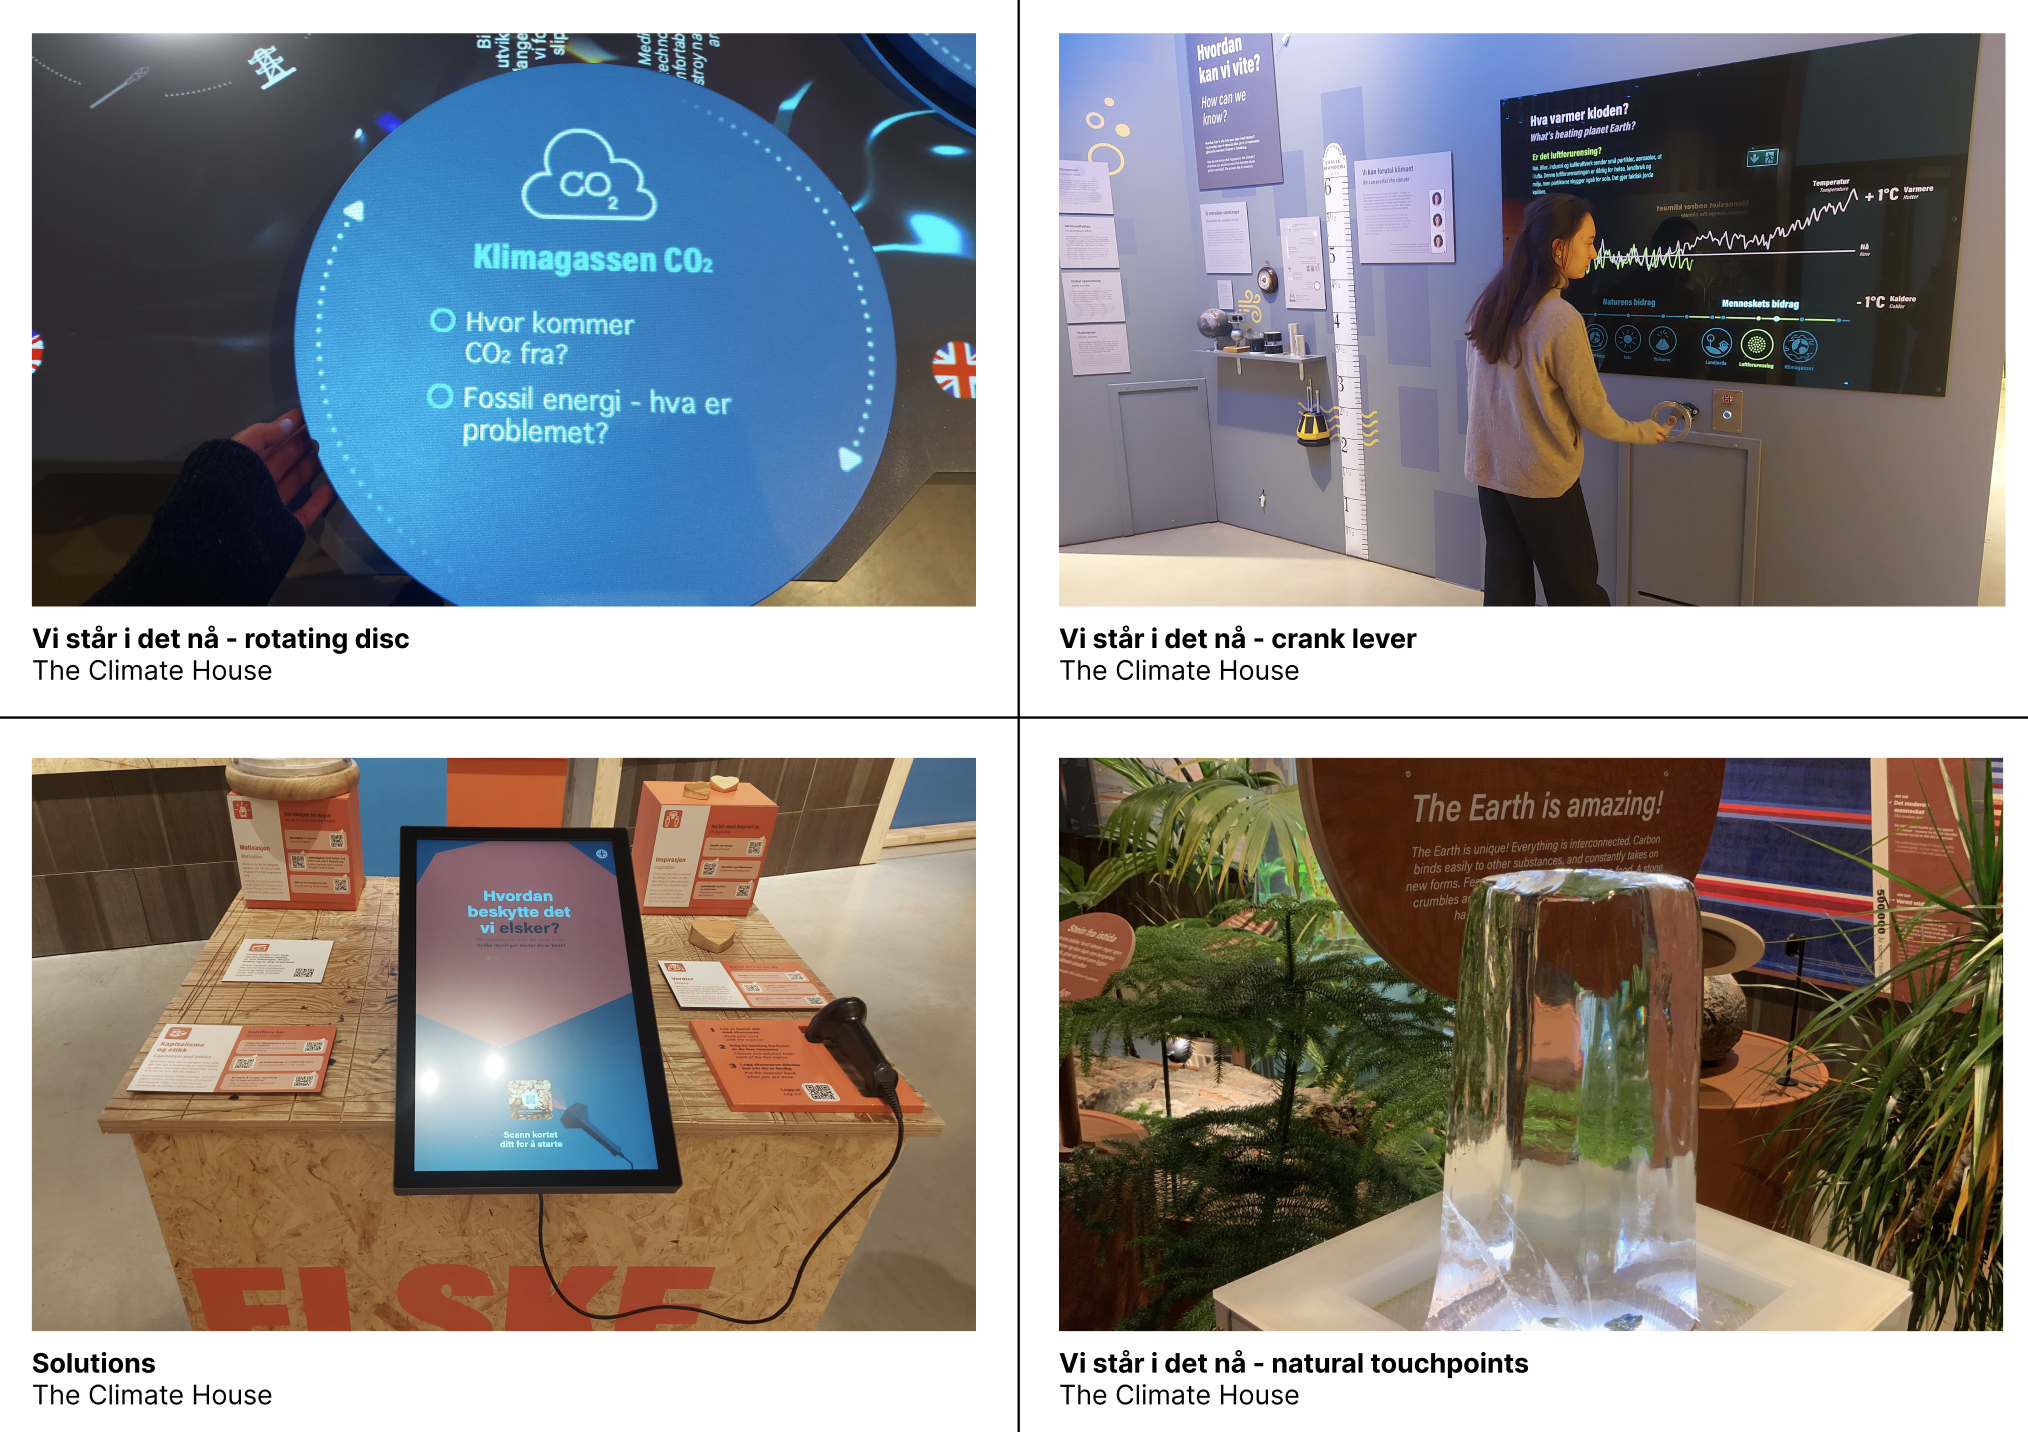
\includegraphics[width=12.5cm]{pictures/klimahuset/klimahuset.JPG}
\caption{Klimahuset}
\centering 
\end{figure}

In the middle of January 2021, covid-19 restrictions started to cease, and we were invited to visit Klimahuset and meet our contact person there for the first time. At the time, Klimahuset was a newly opened museum located in Botanisk Hage at Tøyen in Oslo. Because of strict pandemic restrictions from 12.03.2020 and onward, the museum had only been open for visitors a few months prior to the official lockdown. This visit in January was our first look at the museum space and exhibition \emph{"Vi står i det nå"}, as pictured in Figure 8.2., and we had about 30 minutes to go through the exhibition.

\begin{figure}[H]
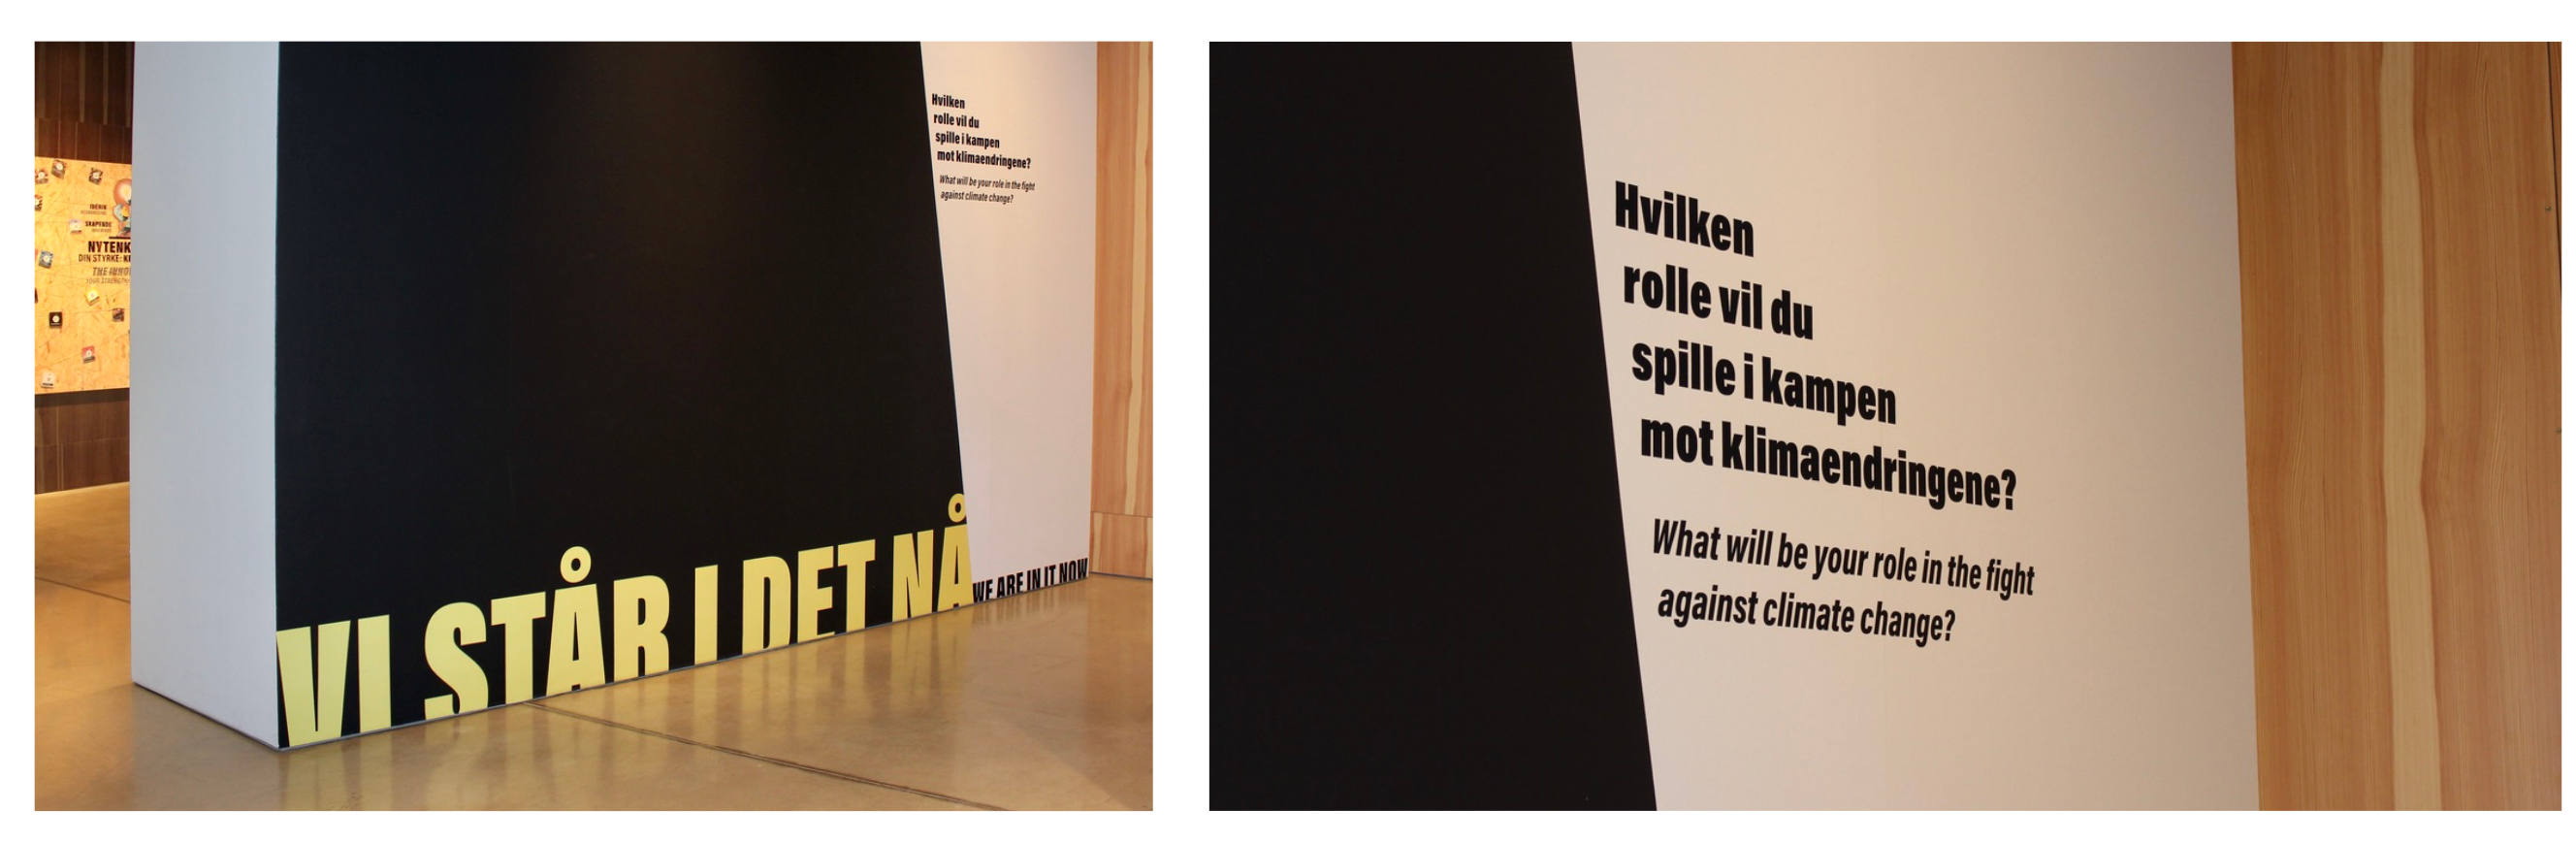
\includegraphics[width=12.5cm]{pictures/process/staar_i_det_naa.png}
\caption{At the start of the exhibition \emph{Vi står i det nå}, they ask; "What will be your role in the fight against climate change?"}
\centering 
\end{figure}

In the aftermath of this first meeting, we were given access to internal documents portraying Klimahusets founding museum values, ambitions, and vision. The documents went in-depth on the exhibition's design process, starting with Klimahusets founding documents, motivation, requirements, and vision for what the museum aimed to address and whom to target. We also got hold of documentation from the design agency responsible for creating the installations, containing both reasoning and documentation of each installation and the proposed optimal visitor journey through the space. The first impression of the exhibition \emph{"Vi står i det nå"} and the founding documents informed our understanding of what an interactive museum context could encompass. As well as what it would mean to design with Klimahuset as the provider of context, not as client.

\begin{figure}[H]
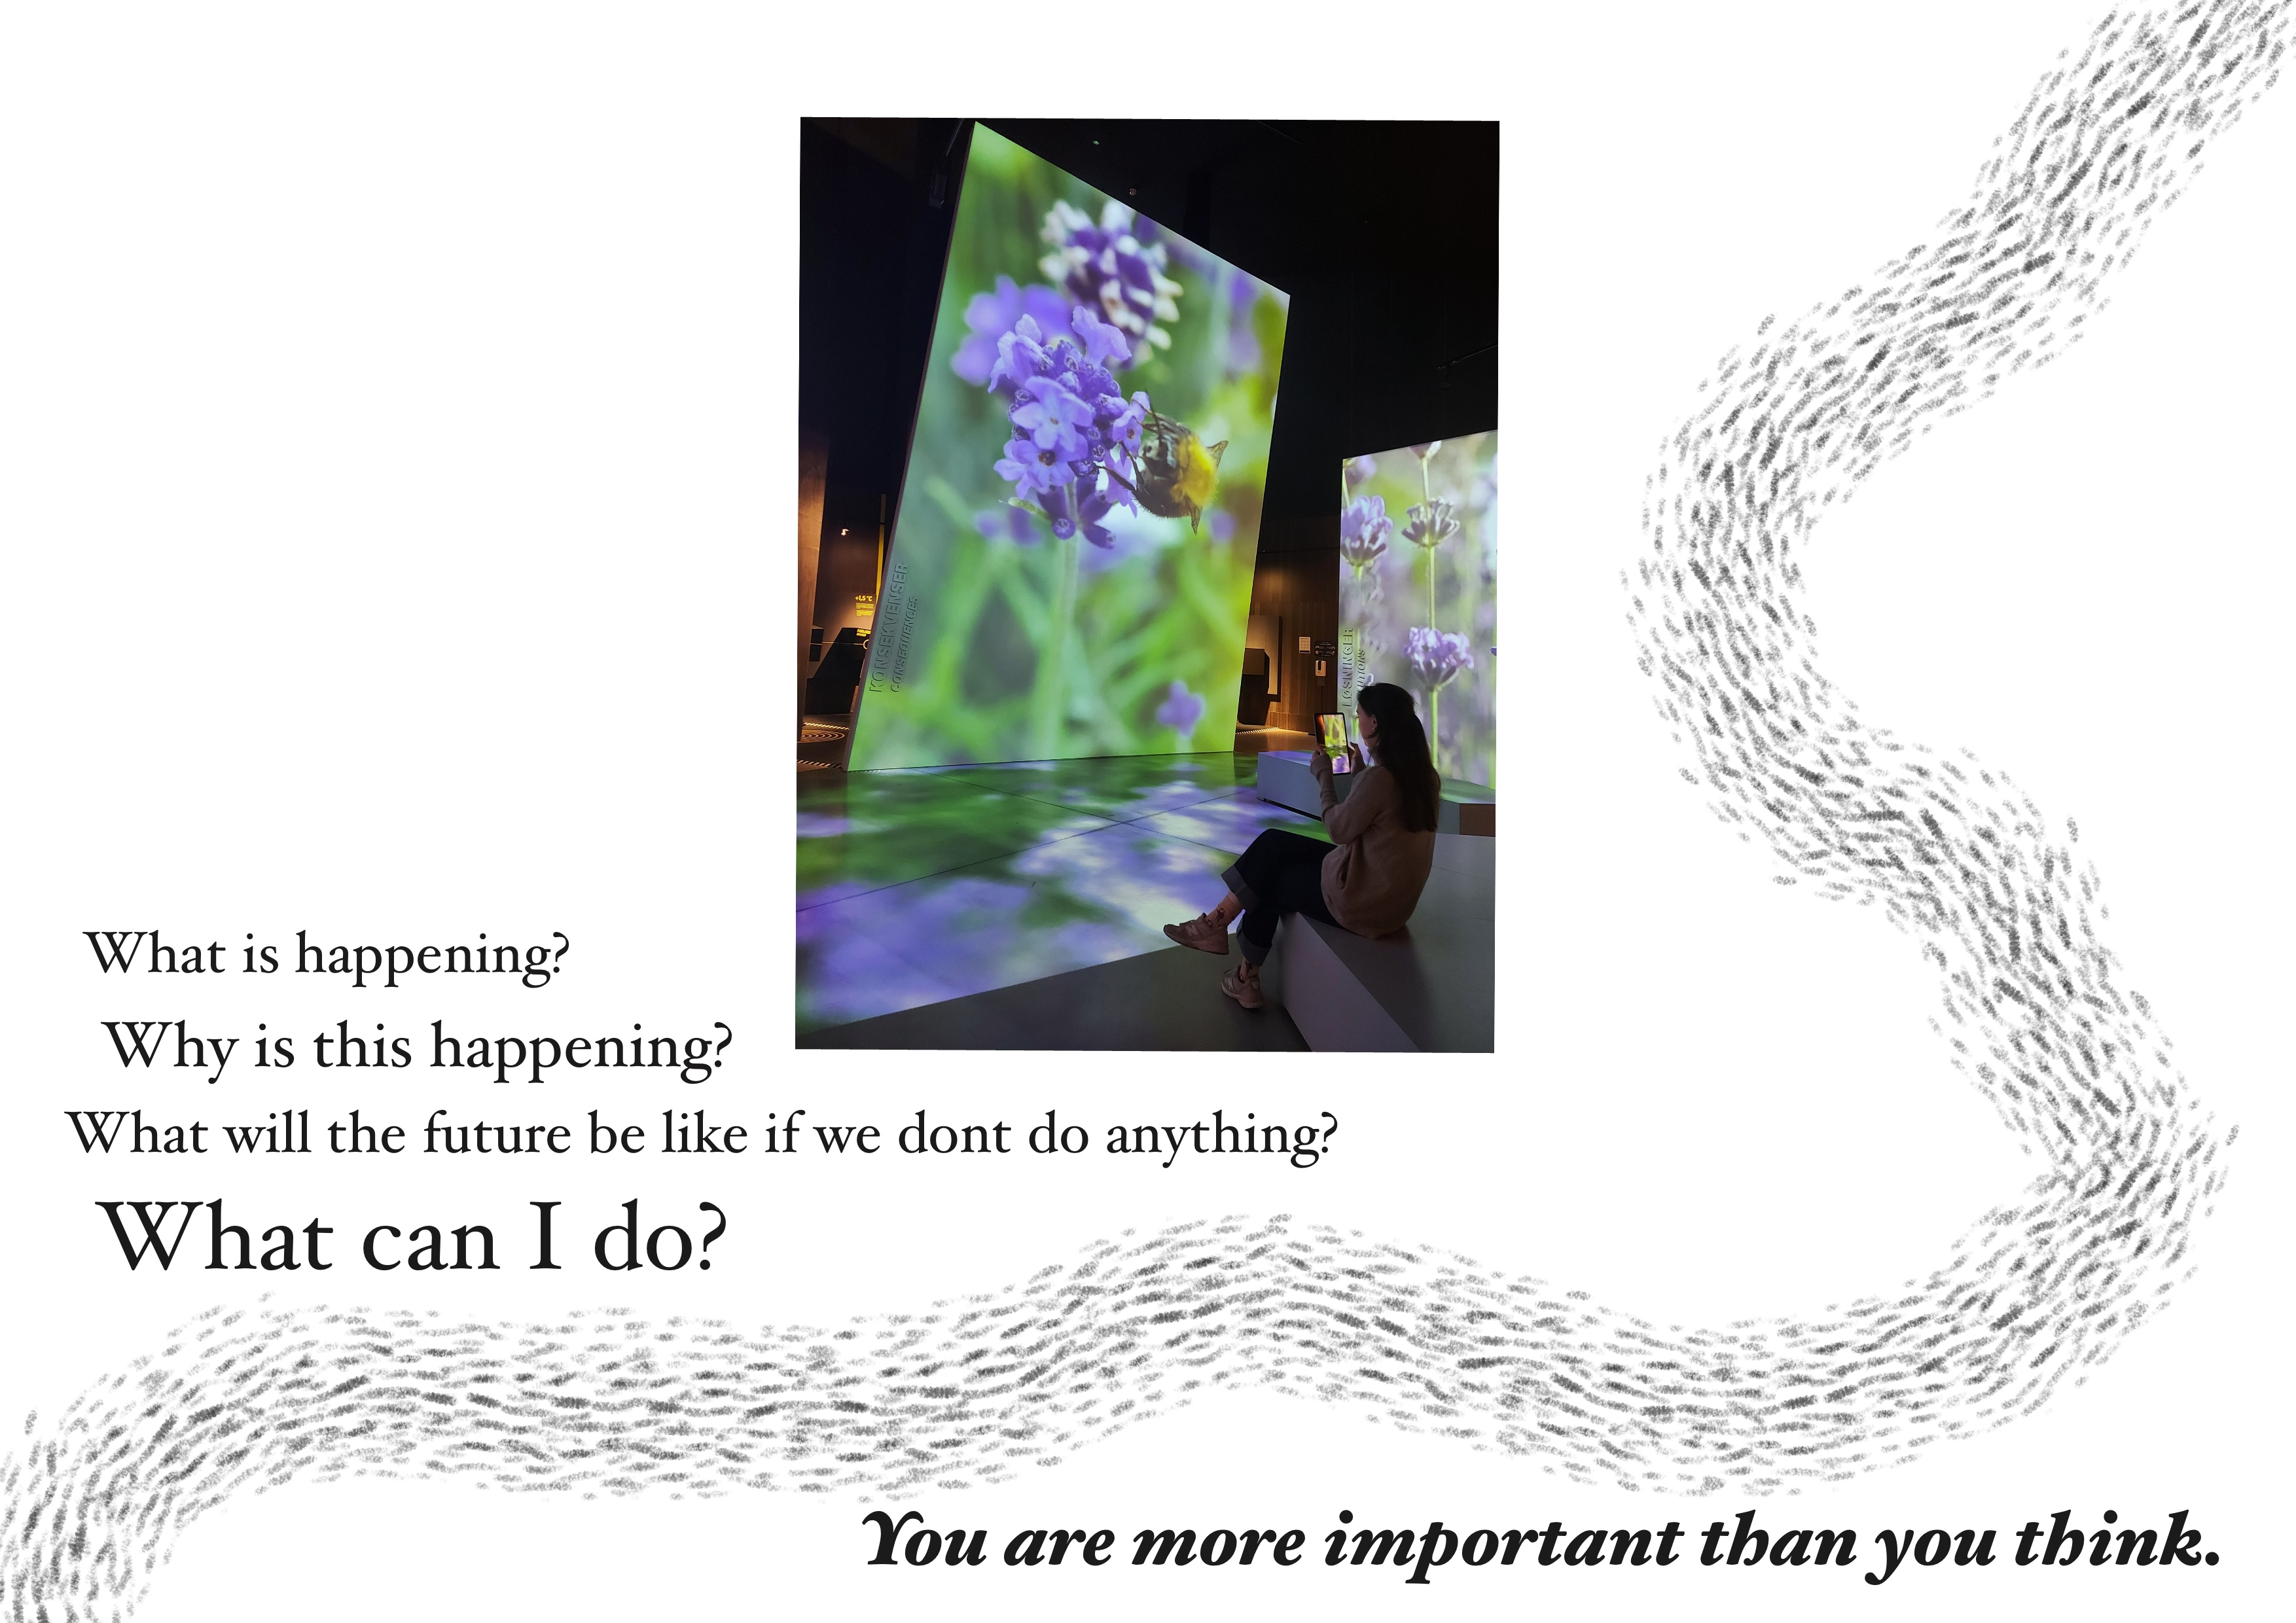
\includegraphics[width=12cm]{pictures/klimahuset/important.jpg}
\caption{Klimahuset want the visitor know that you are an important asset in the fight against climate change, and motivate you to take climate action after the museum visit.}
\centering 
\end{figure}

At this time, the research question I had was quite broad and explorative; \emph{design an interactive visual installation addressing sustainability}. Because the end goal was to create an interactive installation that addressed sustainability, we looked into different topics and values linked to interactivity and sustainability - especially in terms of the interaction designer's role in the climate debate. Walking through a museum is an experience. So it should be, and it is curated as a journey. Drawing inspiration from service-design thinking, we wanted to capture the different elements that made up Klimahusets museum experience. We, therefore, specifically asked for documentation on Klimahuset's values and visions, architecture- or service blueprints, how they collected feedback from visitors and how they measured engagement. The inquiry was driven by the interest in understanding more about how Klimahuset could represent a "modern museum" by studying how they used interactive installations to disseminate, educate, inform and encourage reflections, trains-of-thoughts, conversations, or action with its visitors. Through discussions with the research buddies, we started questioning which areas in the existing space we wanted to do something similar to, and in general, where and how our installation could fit into the existing journey while keeping its integrity and independence. How could we complement and bring a new and different perspective into the exhibition journey? Through these discussions, we defined the following research inquiries:"

\begin{itemize}
    \item Wanted to understand more about how a "modern museum" through the use of interactive installations worked to disseminate and engage with its visitors.
    \item Sustainability is a broad term, wanted to specify it to start conceptual work on the installation. To synthesise the design space.
    \item Where and how will the installation fit into the existing journey, and what will it "bring to the table"?
\end{itemize}

To be able to answer these inquiries, we started to do a literature search and read up on the museum context. The initial reading that started from this point in time is accounted for through Chapter 2-5. We also started conceptual and practical work in parallel with the literature review, preparing to create an installation. The three of us had not fully figured out what kind of research angles we had but agreed that narrative was important, and we were all interested in pursuing sustainability.


\section{Investigating narratives and storytelling with Klimahuset}
\par
\emph{08.04.2021, workshop with members of staff from Klimahuset}
\par

At the start of April 2021, we were requested to host a workshop for different staff members from Klimahuset as a way to kickstart the collaboration with the museum. Inspired by readings on narrative theories and learning in contemporary art museums and the way narratives are constructed in a museum context \autocite{narrative_sitzia}, we saw this as an opportunity to learn more about how narrative play a part in telling a story and in conveying a message. In addition, we wanted the workshop to explore how to engage participants in building a narrative and anticipated that it would give us some insight into building climate-crisis-related narratives. This would also allow us to get some input on which sustainability issues can be a better fit, topic-wise when designing for a learning-oriented type of installation. Lastly, we wanted to facilitate a conversation on the current existing exhibition in Klimahuset, to get some feeling if there were any topics or sustainability issues they wished the current exhibition should address. 

We designed the workshop timeline to endure three phases; brainstorming, storyboarding, and presentation. Because of the ongoing pandemic, we conducted the workshop digitally through Zoom, using Miro as the workshop platform tool. We wanted to get a better grip on different topics and issues in the climate debate that could be used as groundwork for design fiction, so we tried to brainstorm three dimensions that can make up a story; a theme, a dilemma, and a setting. Therefore we asked them:

\begin{itemize}
    \item What topics in the climate debate do you think is important to address?
    \item Write down issues/ dilemmas related to climate debates.
    \item Write down (a climate-related) setting.
\end{itemize}

In the next part of the workshop, we wanted the participants to create their storyboard, where they could choose between all commonly brainstormed themes, dilemmas, and settings - to make up their own story that they would later present. And then, to finalise the workshop, the participants presented their own stories. The stories can be found in the Appendix. It was interesting to see the diversity and different perspectives of the participants and their respective stories. Even though some participants had used the same theme, dilemma, or setting, they all differed in what they wanted to convey with their stories. 

In the aftermath of the workshop, the collected stories and notes from the discussions served as a foundation to look into the relationship between narratives, dissemination in museums, and meaning-making. The main finding I got from the workshop is the notion of how a well-written narrative has the power to make us think about or see ourselves and the Earth around us with new eyes, enabling us to engage in and relate to the climate crisis through the narrative that is told. The climate crisis is a story about humans and humanity, and the power of the narrative lies in the message conveyed.

\begin{figure}[H]
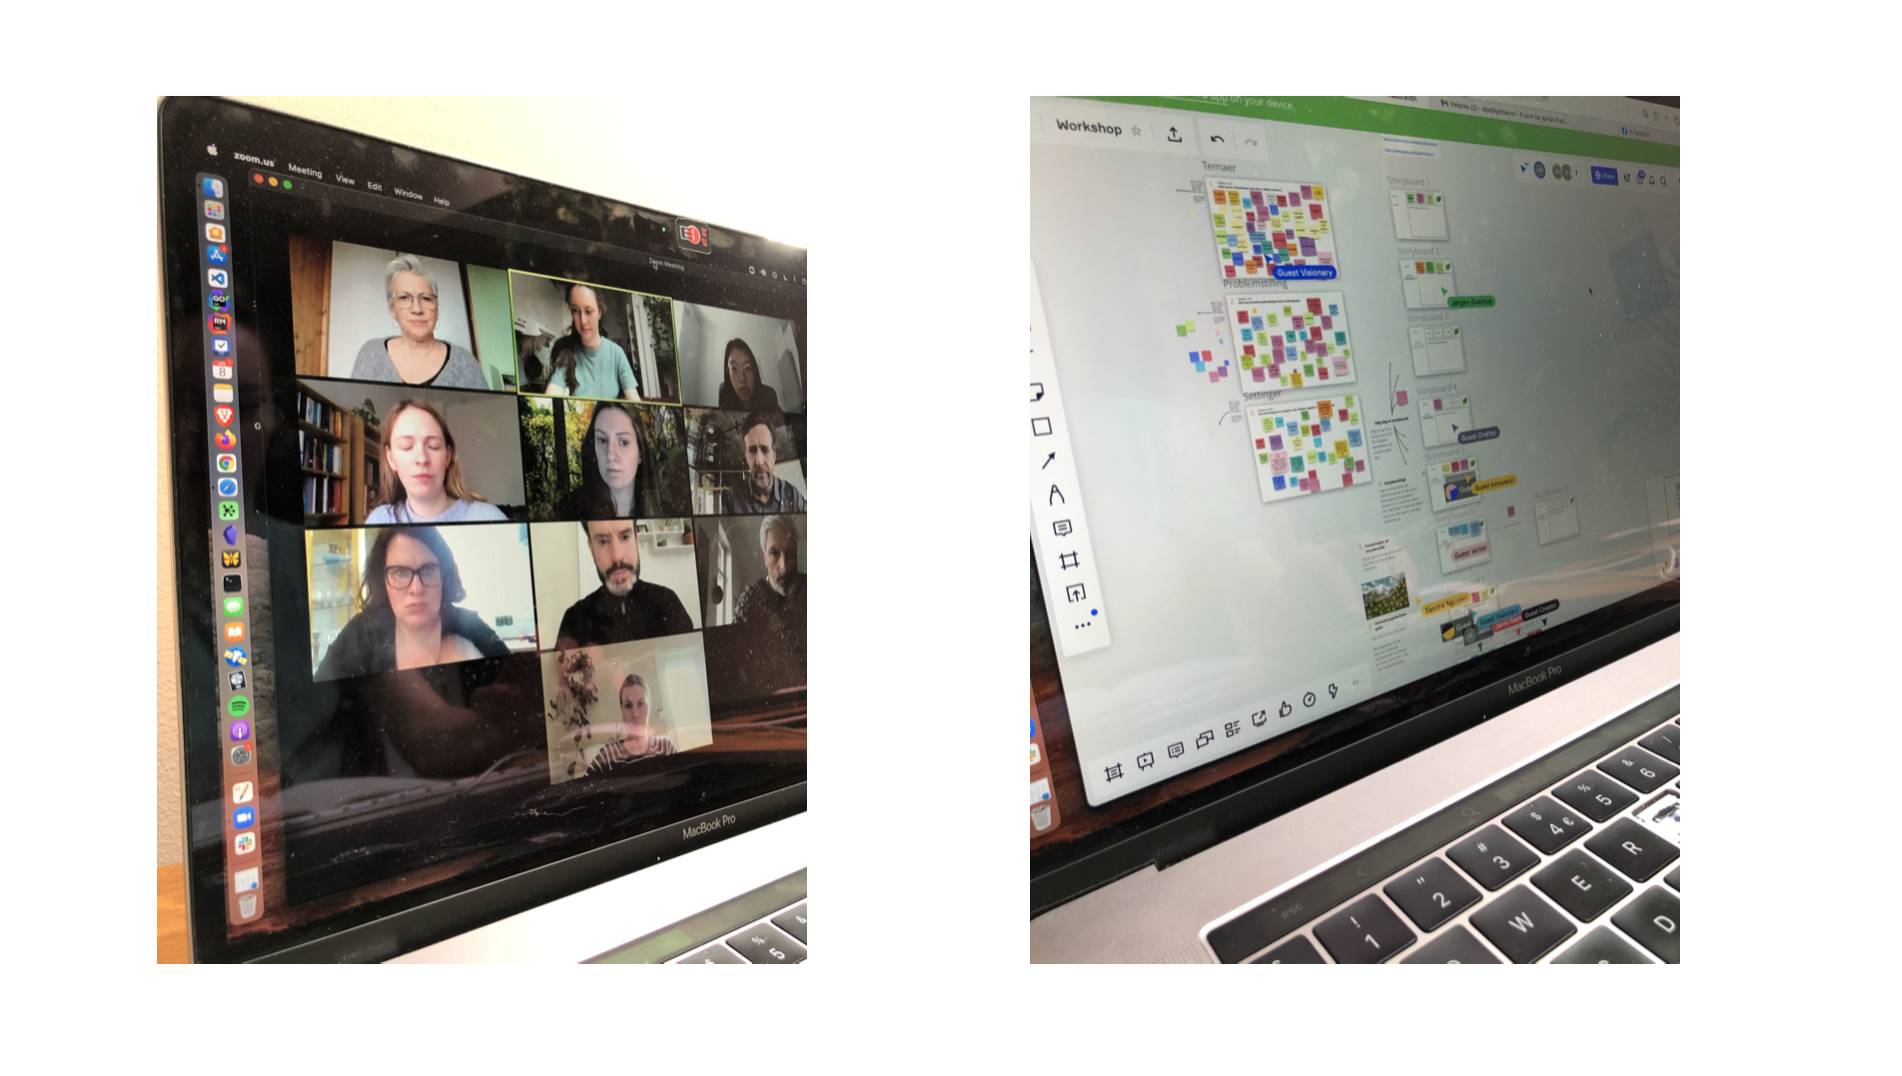
\includegraphics[width=13cm]{pictures/narrative_workshop.png}
\caption{}
\centering 
\end{figure}

\begin{figure}[H]
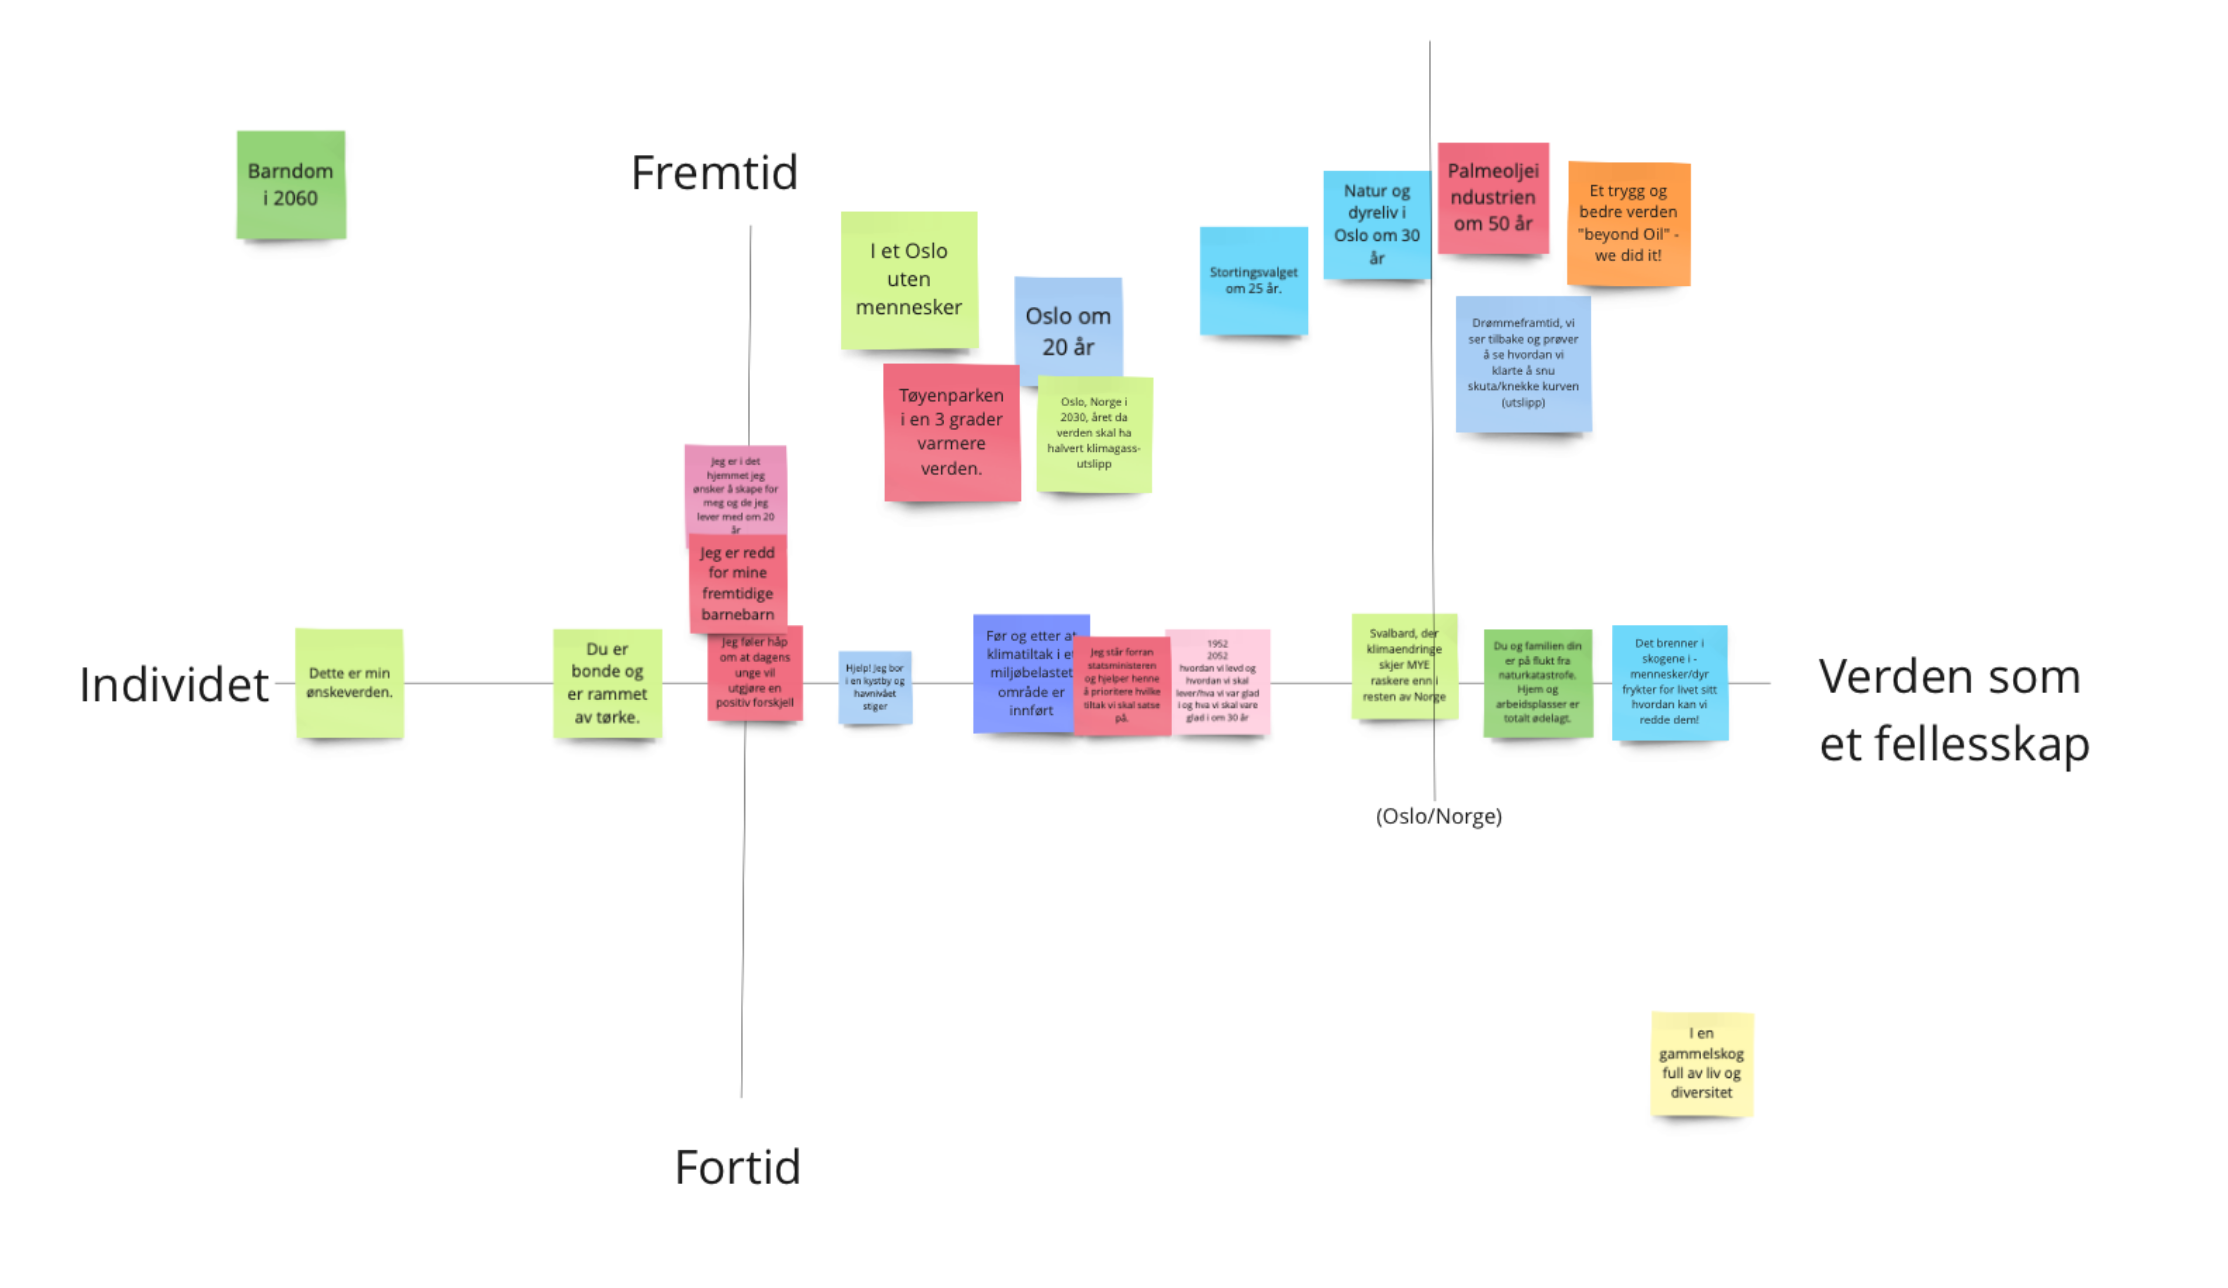
\includegraphics[width=12.5cm]{pictures/process/workshop_results.png}
\caption{}
\centering 
\end{figure}


After the workshop we started conceptualising new ideas and concepts.

\begin{figure}[H]
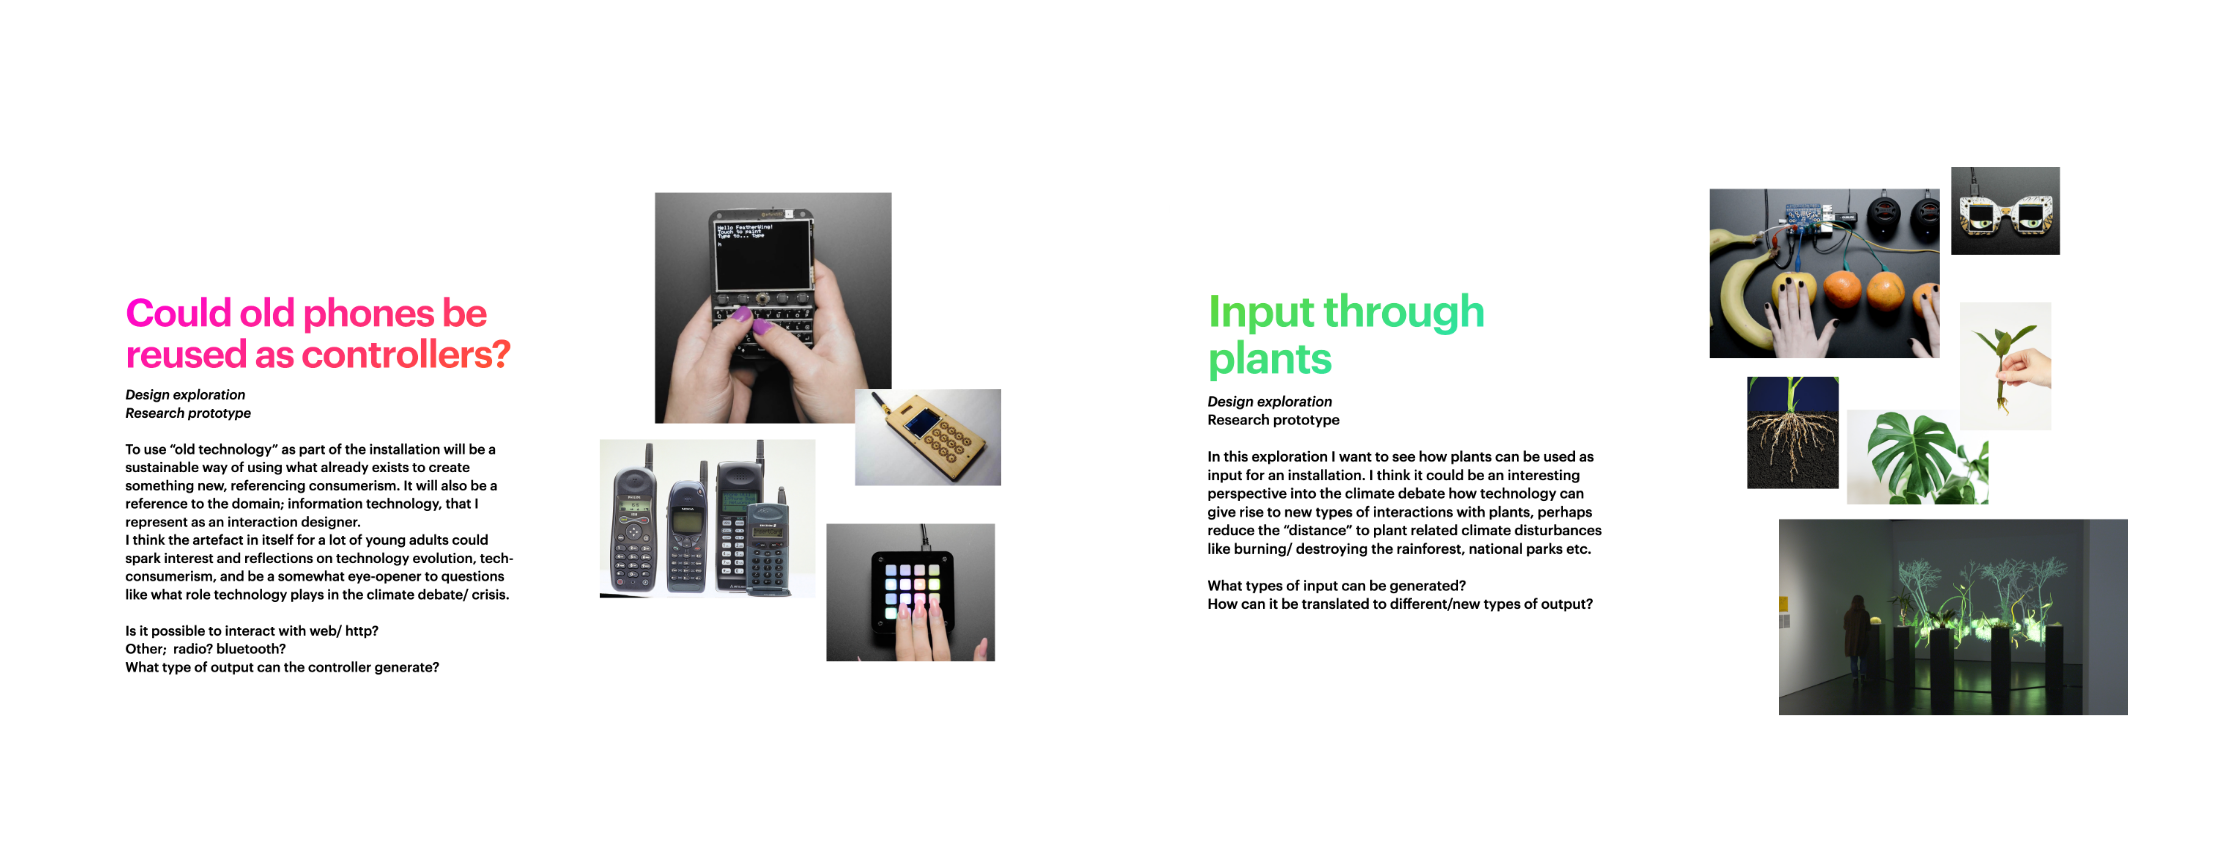
\includegraphics[width=13cm]{pictures/process/mini_pitches.png}
\centering 
\end{figure}



\section{Exploring input through plants}
\par
\emph{01.05.2021, presentation at Klimahuset}
\par

The thought behind this project was to explore how human touch on plants could be used as input, or as a type of controller, to manipulate elements of the installation. The statement of using an actual, living plant would be a direct reference to the relationship between human and nature: plants, animals and ecosystems, bringing nature closer to the discourse where sustainability issues are discussed, inviting to reflections to the ecological damage that we are responsible for. I think this exploration addresses the research question as to how interactive artefacts can provide new depth to the museum discourse, by exploring how human touch through plants can stimulate emotions or values like empathy and awareness, reinforced by the educational environment (the whole museum) the installation is placed in. I believe the plant installation could be interesting to use in combination with learning about plant/ nature related climate disturbances like the burning and destroying of the rainforest, but also in a local, Norwegian context; the windmill debate, hydropower, national park borders, repercussions of cottage development or light pollution. During the shaping of this exploration, I managed to define yet a research question that I want to inquire into; can new/different interactions with natural objects contribute to increased climate consciousness and activism?	

\begin{figure}[H]
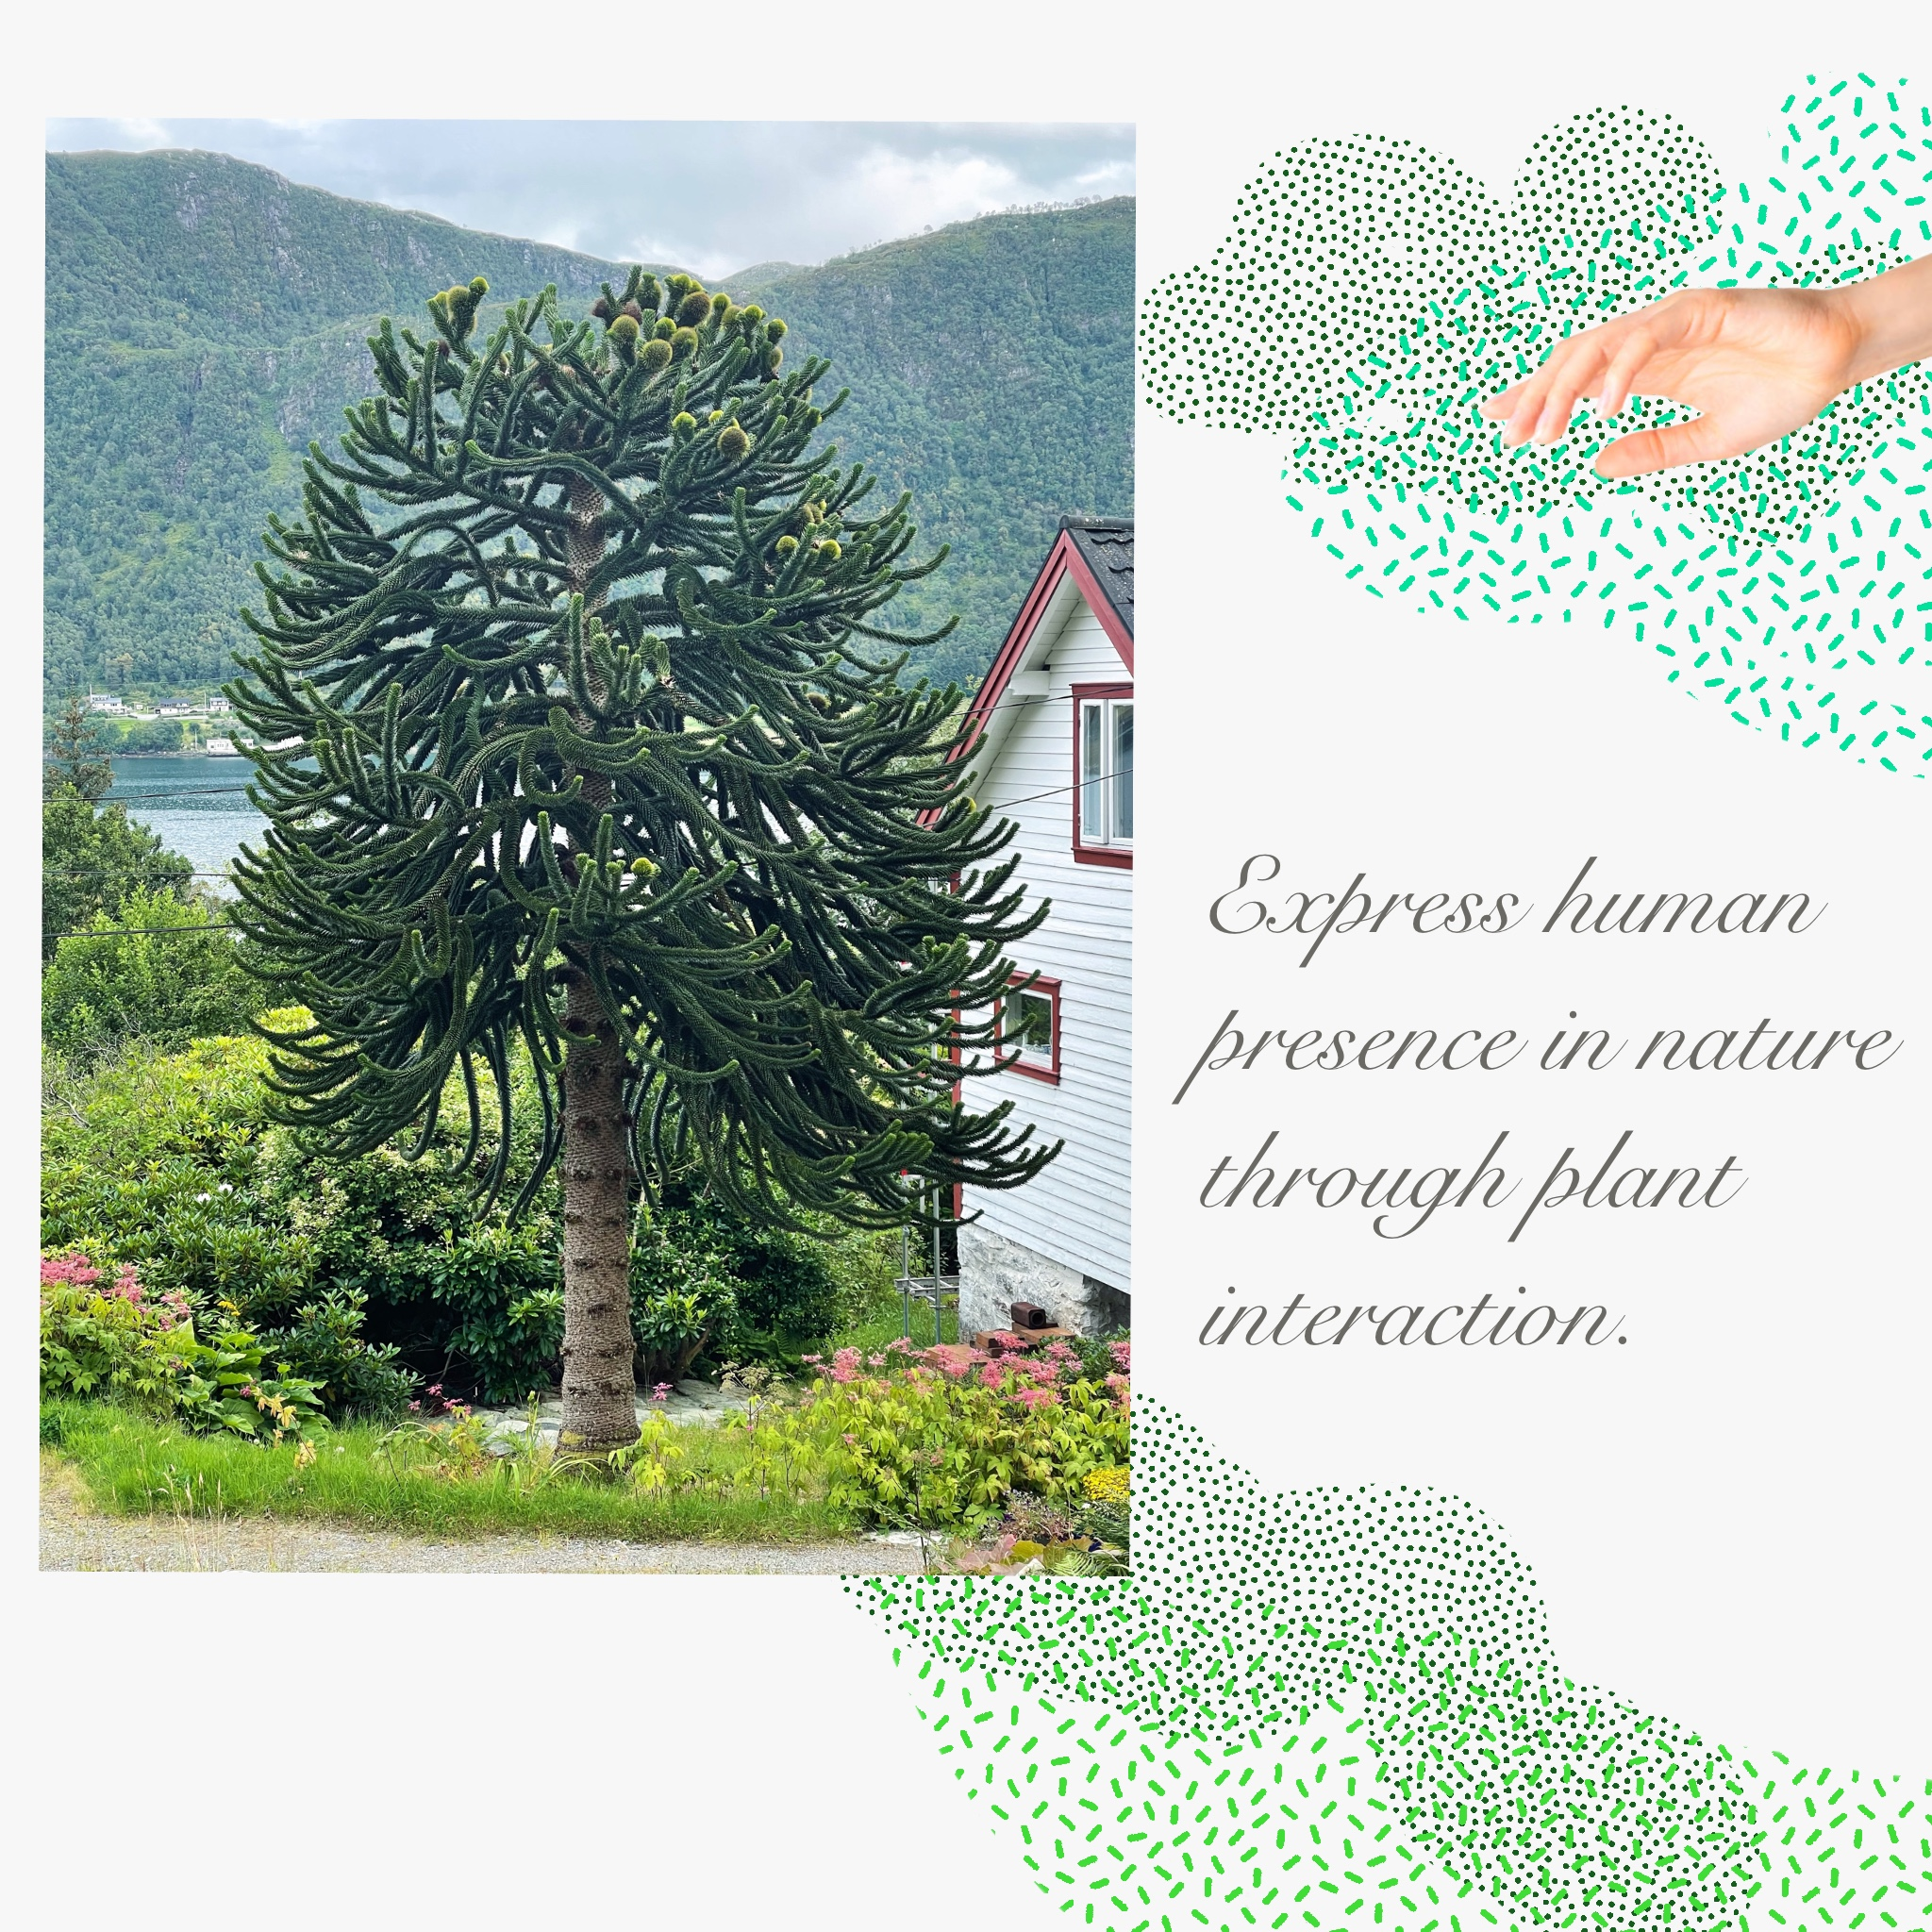
\includegraphics[width=13cm]{pictures/human_presence.jpg}
\centering 
\end{figure}


\section{Slow Design exhibition}
\par
\emph{25.08.2021-01.10.2021, tangible interaction intensive course}
\par

In September 2021 I took part in an intensive studio course called Tangible Interaction (IN5470). Each year, a theme is given that the students explore in a project that spans over the course of five weeks. This year's theme was Slow Design, and in groups of three we were challenged to design and create a fully operational installation by the end of the course, and unveil the installation in a joint exhibition along with the other groups. 
% Legge inn noe om Slow Design, trekke inn noen artikler kanskje? Eller bare reflektere rundt lærdommer fra temaet, og hvordan det påvirket videre prosess. Det er etter Tangible at jeg/ vi går vekk fra å lage en egen installasjon til masteroppgaven, både på grunn av tidspress, og på grunn av Torkjell (selv om jeg tenker å ikke nevne det).

\subsection{Memento Mori}

\begin{figure}[H]
\includegraphics[width=12cm]{pictures/process/memento_mori.pdf}
\caption{Memento Mori concept pitch}
\centering 
\end{figure}

Memento Mori was exhibited in the joint exhibition \emph{Slow Design: Reveal}. The installation was placed in a small room. One of the team members worked as a docent getting visitors in groups of 3-4 people in and out of the room. Windows covered with black fabric, a forest-scented candle and a pink flower was placed on a table in the corner next to the installation who covered almost the whole wall. On the table there was placed three or four books with an old-fashioned ornamental style. Another team member was sitting by the table by the candle - operating the technicalities of the installation and welcoming us.

"Which one of you want to take a leaf out of the basket?", we were asked, and one eagerly stepped forward to the person holding the basket. 




\subsection{Presence in Existence}

\begin{figure}[H]
\includegraphics[width=10cm]{pictures/process/presence_in_existence.pdf}
\caption{}
\centering 
\end{figure}

\subsection{Qi}

\begin{figure}[H]
\includegraphics[width=10cm]{pictures/process/qi.pdf}
\caption{}
\centering 
\end{figure}


\section{I/O (In Oslo) by Yuko Mohri}
\par
\emph{22.10.2021, excursion to Atelier Nord}
\par

In late October, me and my research buddies visited Atelier Nord to see and analyse the ongoing exhibition by Yuko Mohri: I/O (In Oslo). Going in, we expected the exhibition to be or have interactive qualities, and my research interest during this fieldwork was guided by \autocite{hybridplace_ciolfi}'s Hybrid Place dimensions. 

This is how Atelier Nord describes the installation: 
\emph{Gently cascading rolls of paper are fixed to a framed structure in the ceiling and pick up dust and other debris. The traces are scanned and converted into random input-output signals that case a constellation of objects, such as feather dusters and old musical instruments, to move and produce sound. The site-specific characteristics - including movements of air, humidity, and the undulating surface of the floor - are picked up by the rolls of paper, gradually permeating it with the unique features of the exhibition space. The result is an organic environment where the same sound and movement never occurs twice. In this case, the gallery might be likened to a biotope-like ecosystem that interweaves the natural and artificial.} \autocite{yukomohri_web}

What follows is an experience account from my visit. Guided by the Hybrid Place framework, I first looked for the physical and structural qualities of the space. I noted how the showroom was large, kind of empty and very open. The installation itself consisted of two separate installations, both placed in the center of the room, so that visitors could walk both around and in-between the two installations. There was also a small room where the visitor could see a movie about Yuko Mohri and her thoughts behind the installation. There was no tape on the floor, or signs saying to not touch or walk, and in that sense the showroom invited to make our own path and discover the installation in our own pace and way we wanted. The showroom was pretty small, perhaps around 30kvm, and aesthetically quite plain. The wooden floor creaked when walking, and the sound echoed through the space. There was no music or what-so-ever in the background, only faint city-noises from one side of the housing and rustling of leaves from the other. The installation produced sound randomly from two outputs; feather dusters and an old musical instrument. During our visit we only heard the thumping from the feather dusters you can see depicted above. I noted how "clacking" sounds from both my own and other visitors shoes directed the attention toward movement in the room. The effect were especially reinforced after standing still for a while, looking, thinking about the installation. I noted that in the moment, sound and movement produced by the other visitors in the room influenced my mental presence being drawn back-and-forth, in-and-out, from the mind-space I was present in when observing and thinking about the installation, and then drawn back again to the physical space. Because of the showrooms atmosphere as I just described, and the room being small, it's easier to meet eye-to-eye with the other visitors, listen in on their conversations, and simply being aware of their presence. It felt a little awkward to talk, and sometimes also to move, resulting in a quiet/ whispering way of communicating with my research buddies during the visit.

\begin{figure}[h]
    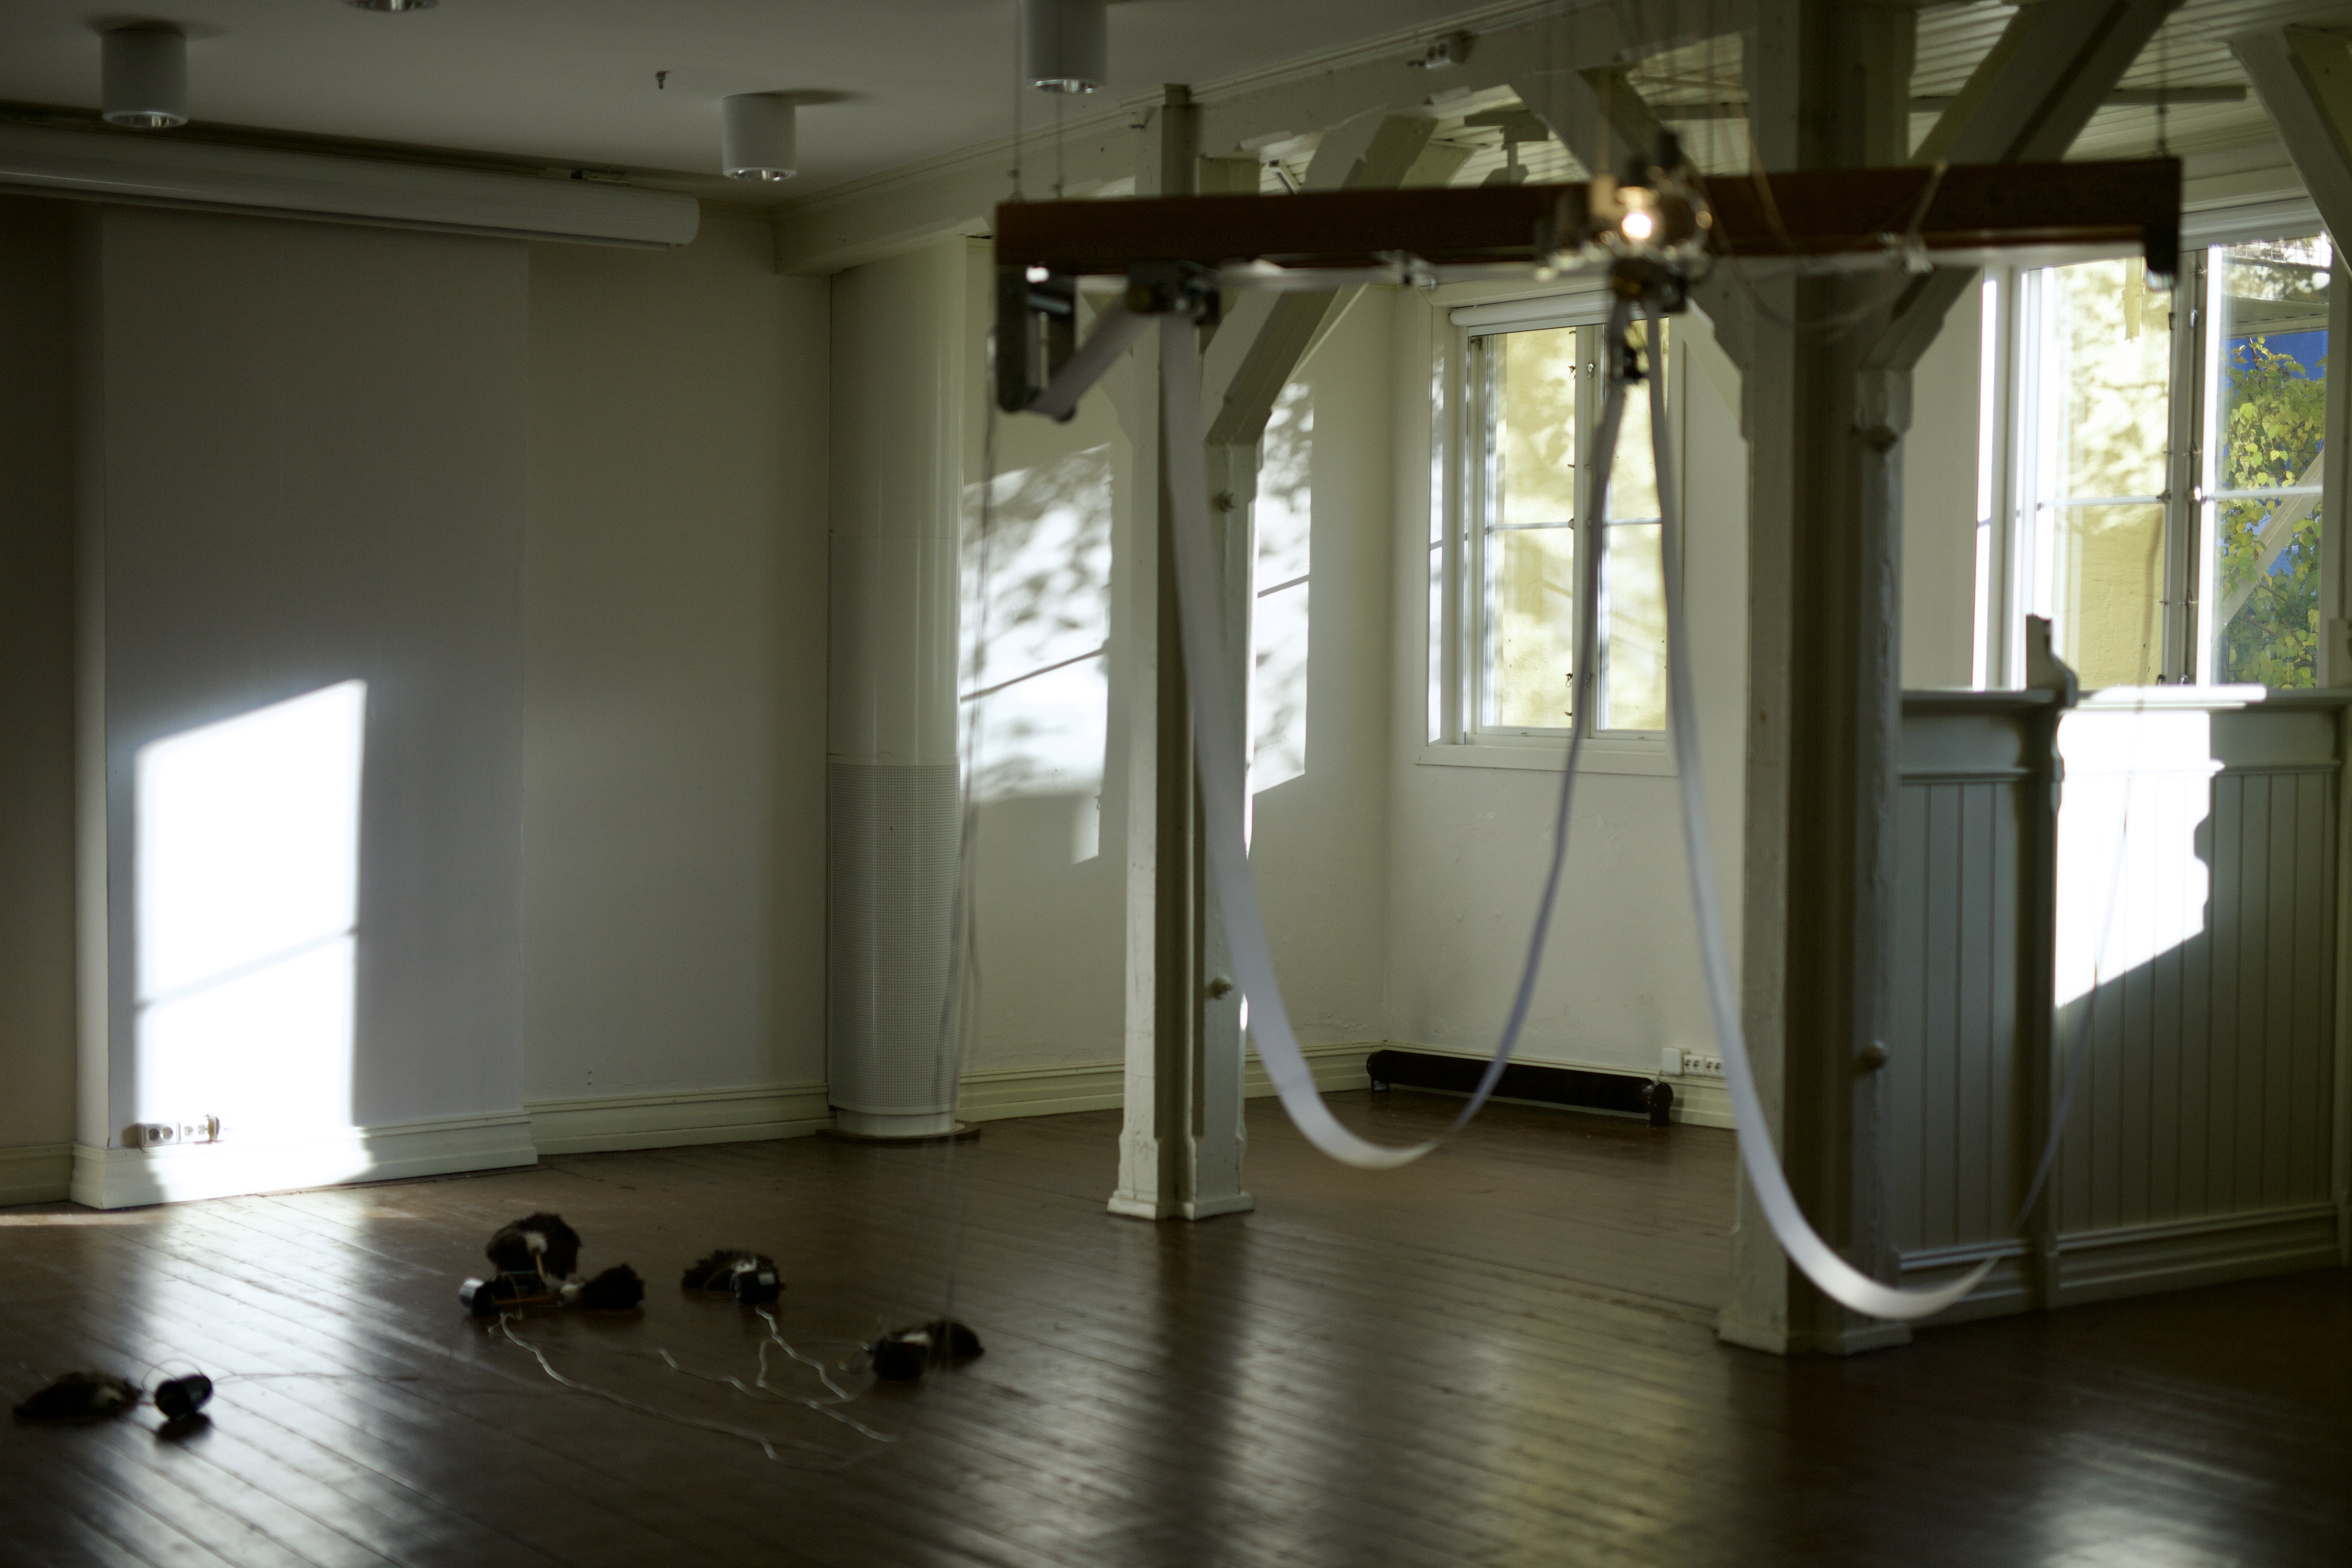
\includegraphics[width=12cm]{pictures/process/yuko_harmony.jpeg}
    \centering 
    \caption{Notice how the sunlight add a layered meaning to traces in the air being picked up by the cascading rolls of paper.}
\end{figure}

In terms of the physical/ structural dimension \autocite{hybridplace_ciolfi}, I would say that the space support group interactions, but it doesn't favour it. Therefore, I noted that the exhibition did not fit into the social dimension of the Hybrid Place framework. Coming into the showroom in a group of three, we actually had the space to ourselves for quite some time, but we walked around in silence for most of that time. Eventually, two people entered, and we were then not alone. Because we already had been there a while, we shifted focus from the details in the installation and how it worked, to see how the pair moved around and used the space. The presence of a new group of people did not change the atmosphere as I described, they were also walking slowly, talking in a quiet manner and payed attention to the way we moved around the installation as well. Perhaps they assimilated us, or the atmosphere we created? I actually did not notice the video-room before these two new people entered, as this was the first thing they did after talking to the Docent and orienting themselves in the space.

When it comes to the last two dimensions, the cultural and personal dimension \autocite{hybridplace_ciolfi}, I have only categorized the 

+ personal
+ cultural


\begin{figure}[H]
\includegraphics[width=12cm]{pictures/process/yuko_presence.jpeg}
\centering 
\end{figure}

The Docent who was in charge of the space and exhibition was quiet, looked tired, and did not initiate any dialogue or conversation about the installation. We were kind of just left to ourselves the entire time.

\begin{comment}
\begin{figure}[H]
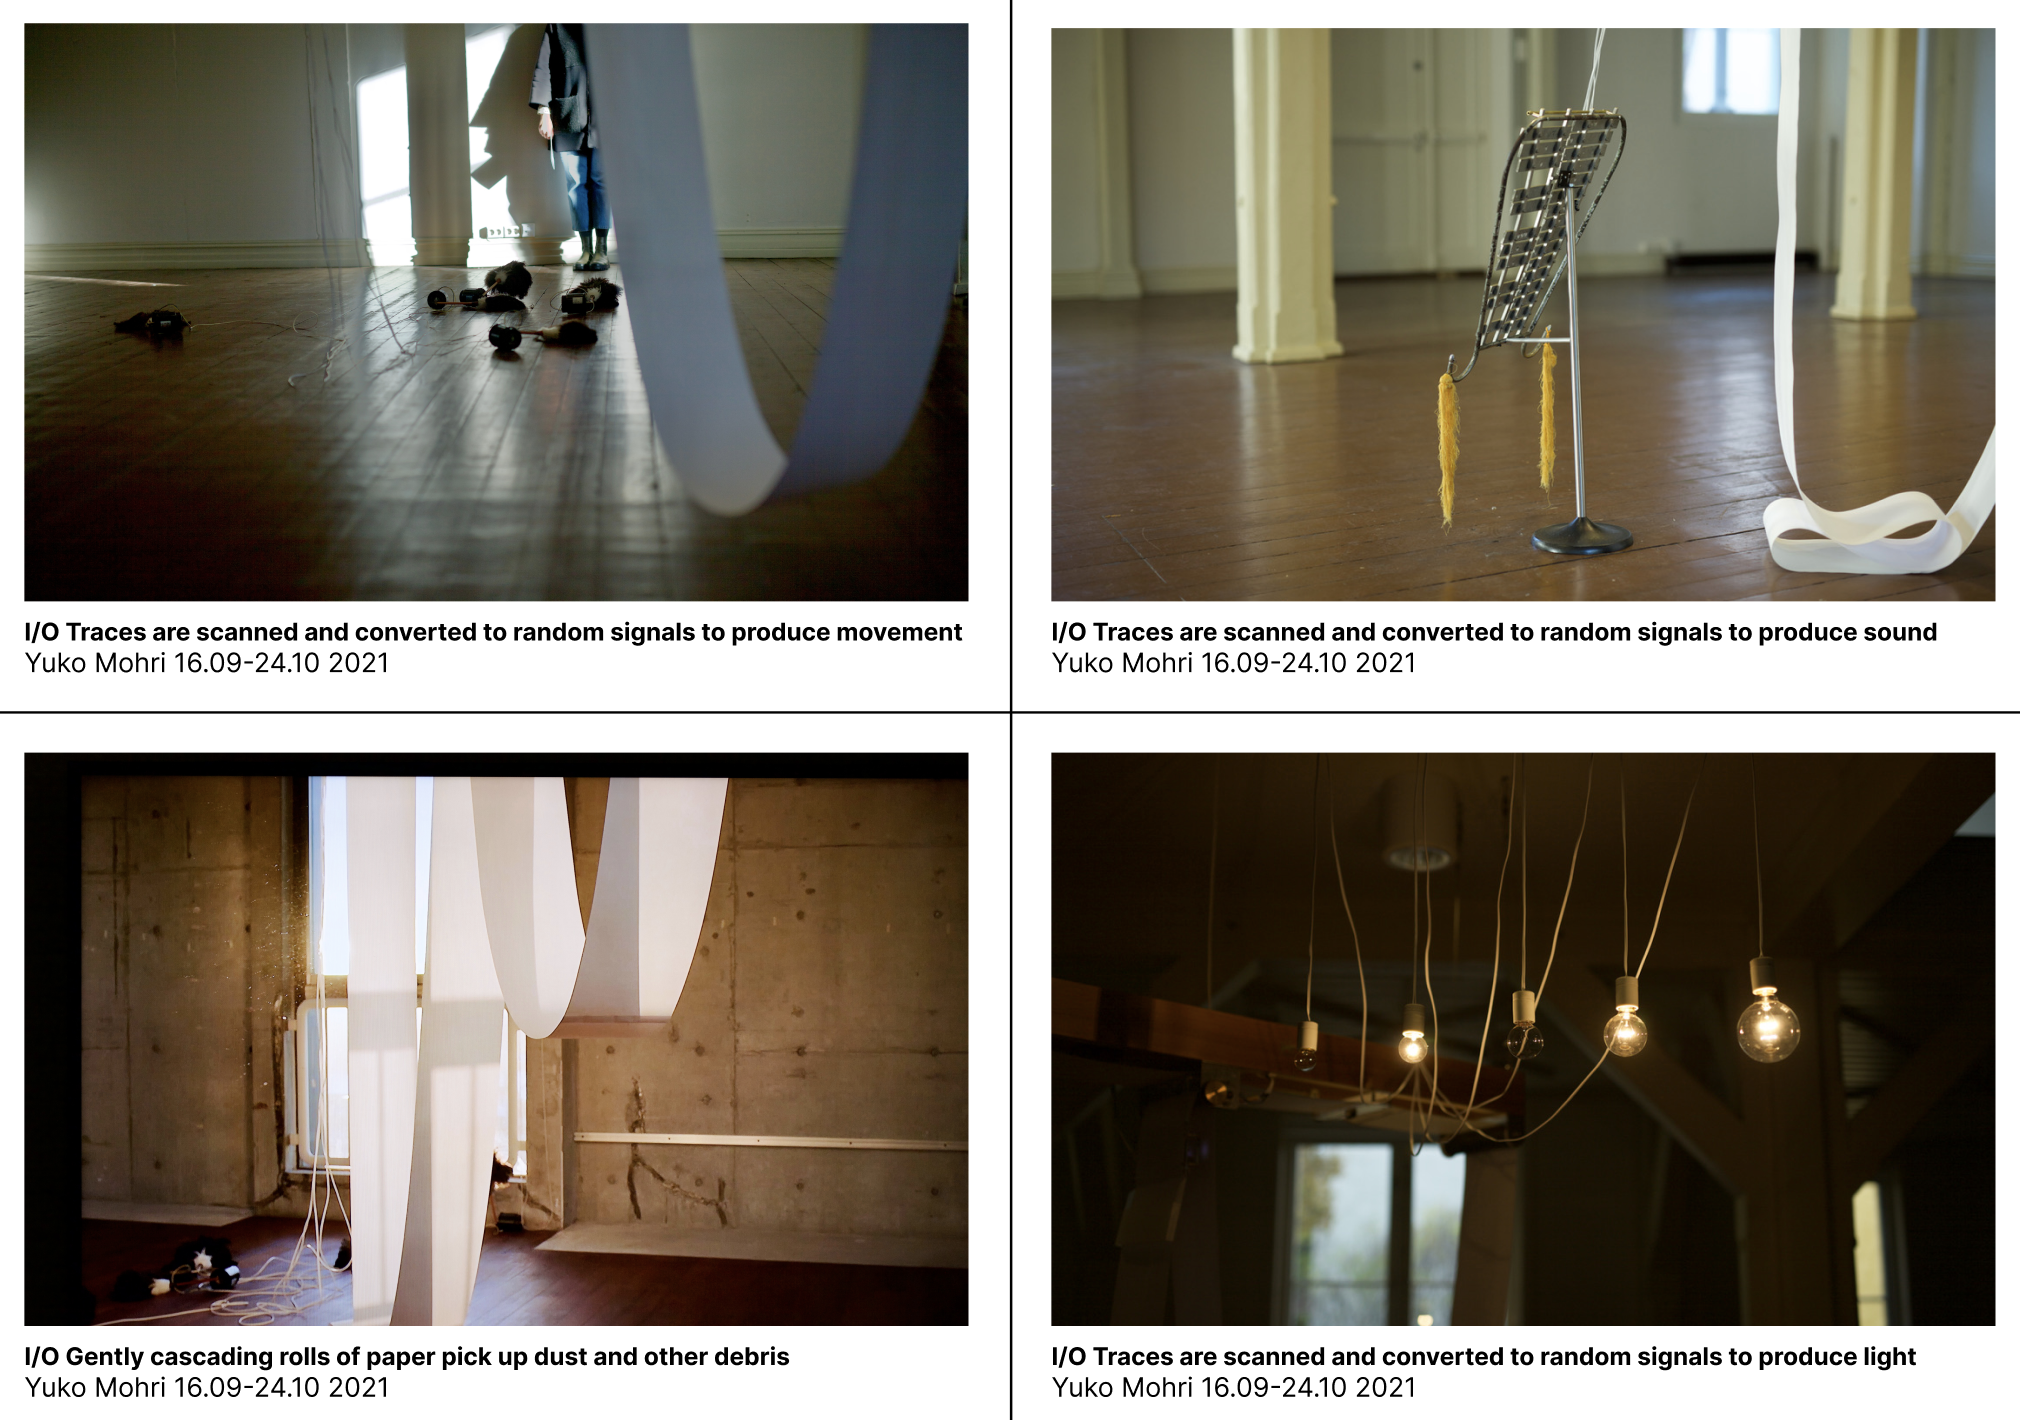
\includegraphics[width=12cm]{pictures/dataset/yuko_mohri.png}
\centering
\end{figure}
\end{comment}

\section{Poison: An Edvard Munch Experience}
\par
\emph{27.10.2021, excursion to Munch Museum w/ focus on the interactive experience Poison}
\par

A couple of days after we visited I/O (In Oslo) by Yuko Mohri, we went to see the newly opened MUNCH Museum in Bjørvika, Oslo. The MUNCH museum is a stereotypical example of an art museum, exhibiting and showcasing Edvard Munch's art, his life and the state of the society and culture from when he lived. We had read that there was to be exhibited a temporary interactive exhibition called Poison: An Edvard Munch Experience. This is how MUNCH describes the exhibition: \emph{"Poison: An Edvard Munch Experience leads you down to the murky depths of Munch’s art, into a painted world of unreliable stories and shifting perspectives. This is achieved through the use of floor-to-ceiling video projections, AI-powered morphing visuals, movement tracking, light experiments, and spatial sound. The technology gives life to a mysterious being that produces a never-ceasing maelstrom of hypnotic imagery, a being that is always on the move and that responds to each step that you make. Do you dare to explore the enigma of Munch’s green-tainted world?"}\autocite{munch_poison_web}

\begin{figure}[H]
\includegraphics[width=12cm]{pictures/process/poison_poisonous.png}
\caption{Poison: An Edvard Munch Experience}
\centering
\end{figure}

What follows is an experience account from my visit, where what I have been looking for is guided by the Hybrid Place framework. The exhibition was located on the 6th floor, and a Docent was standing by the entrance letting in a few people at a time. The first room we entered was a hallway-like rectangular room with an illuminating pink wall with written text introducing the theme. The floor had a soft, black carpet which muffled the sound from our feet - a contrast to the hard wooden flooring found in the other exhibitions. I noted sounds and a kind of creepy ambience from the next room, and while reading starting to build up anticipation for what awaited. A bit restless, I eagerly moved into the next room. The room had floor-to-ceiling video projections on three of the walls, projecting blurred and flickering Munch paintings. I was pretty sure I had seen some of the paintings briefly before, but did not recognise any of them like I can with other Munch paintings. Being kind of color-blind from the pink room, the first impression of this new room was quite overwhelming - to begin with the colors really "popped" and were really saturated, especially the greens. Eventually the eyes adjusted, in probably just a few seconds, for the color-scheme to fade into a more dim and corpse-like, nauseous and "sickening" palette. The sound-landscape accompanying the projections is hard to describe; it seemed like noises were synced with the projections, so that when the picture went in- or out-of-focus or flickered, crackling and sizzling noises accompanied it. Simultaneously there were low-pitched undertones in the background creating the base for a dark and mystic atmosphere.

\begin{figure}[H]
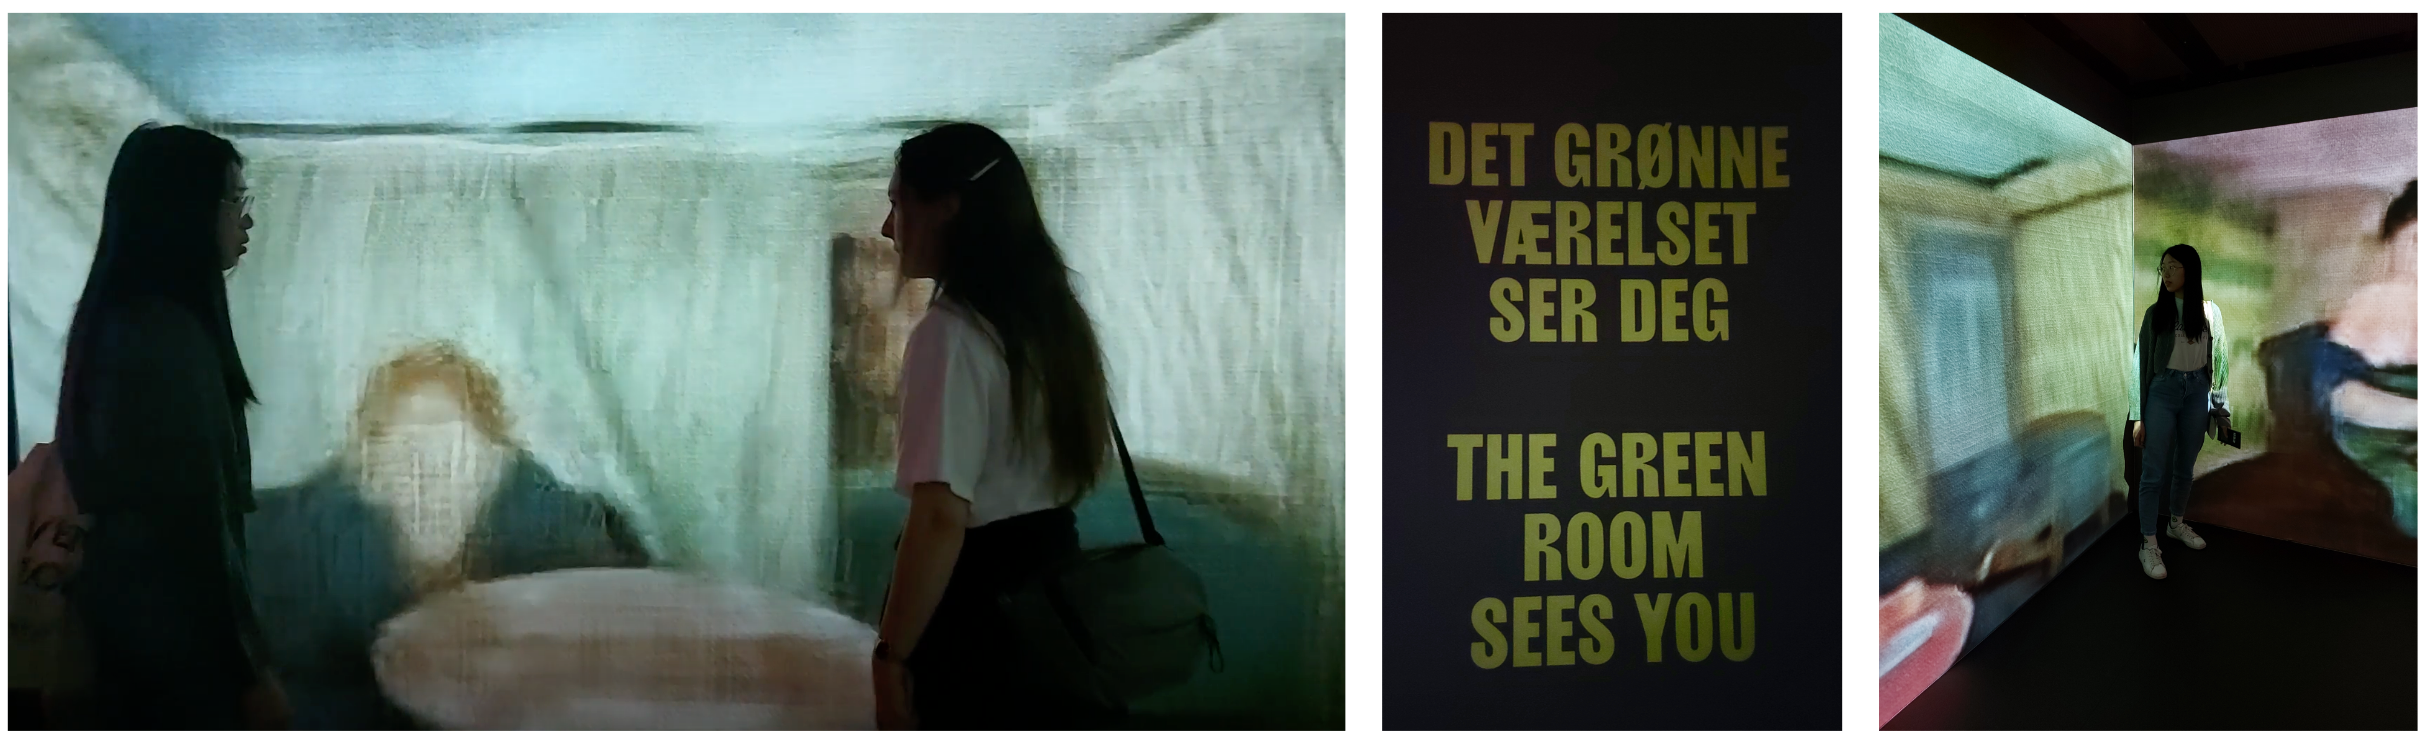
\includegraphics[width=12.5cm]{pictures/process/poison_seeu.png}
\caption{Poison: An Edvard Munch Experience}
\centering
\end{figure}

In terms of the social dimension I would say that the exhibition opens for some social interaction to take place, e.g. you can whisper to eachother and have a low-pitched somewhat private conversation on what you see - but there is no explicit dialogic qualities. The projections and sound-landscape creates an immersive experience, which I would say really emphasises the personal dimension. A combination of the written emphasis on \emph{the green room}, as well as the distinct color-scheme in the chosen paintings projected; have in the aftermath of the visit been what I distinctively remember. 

\begin{figure}[H]
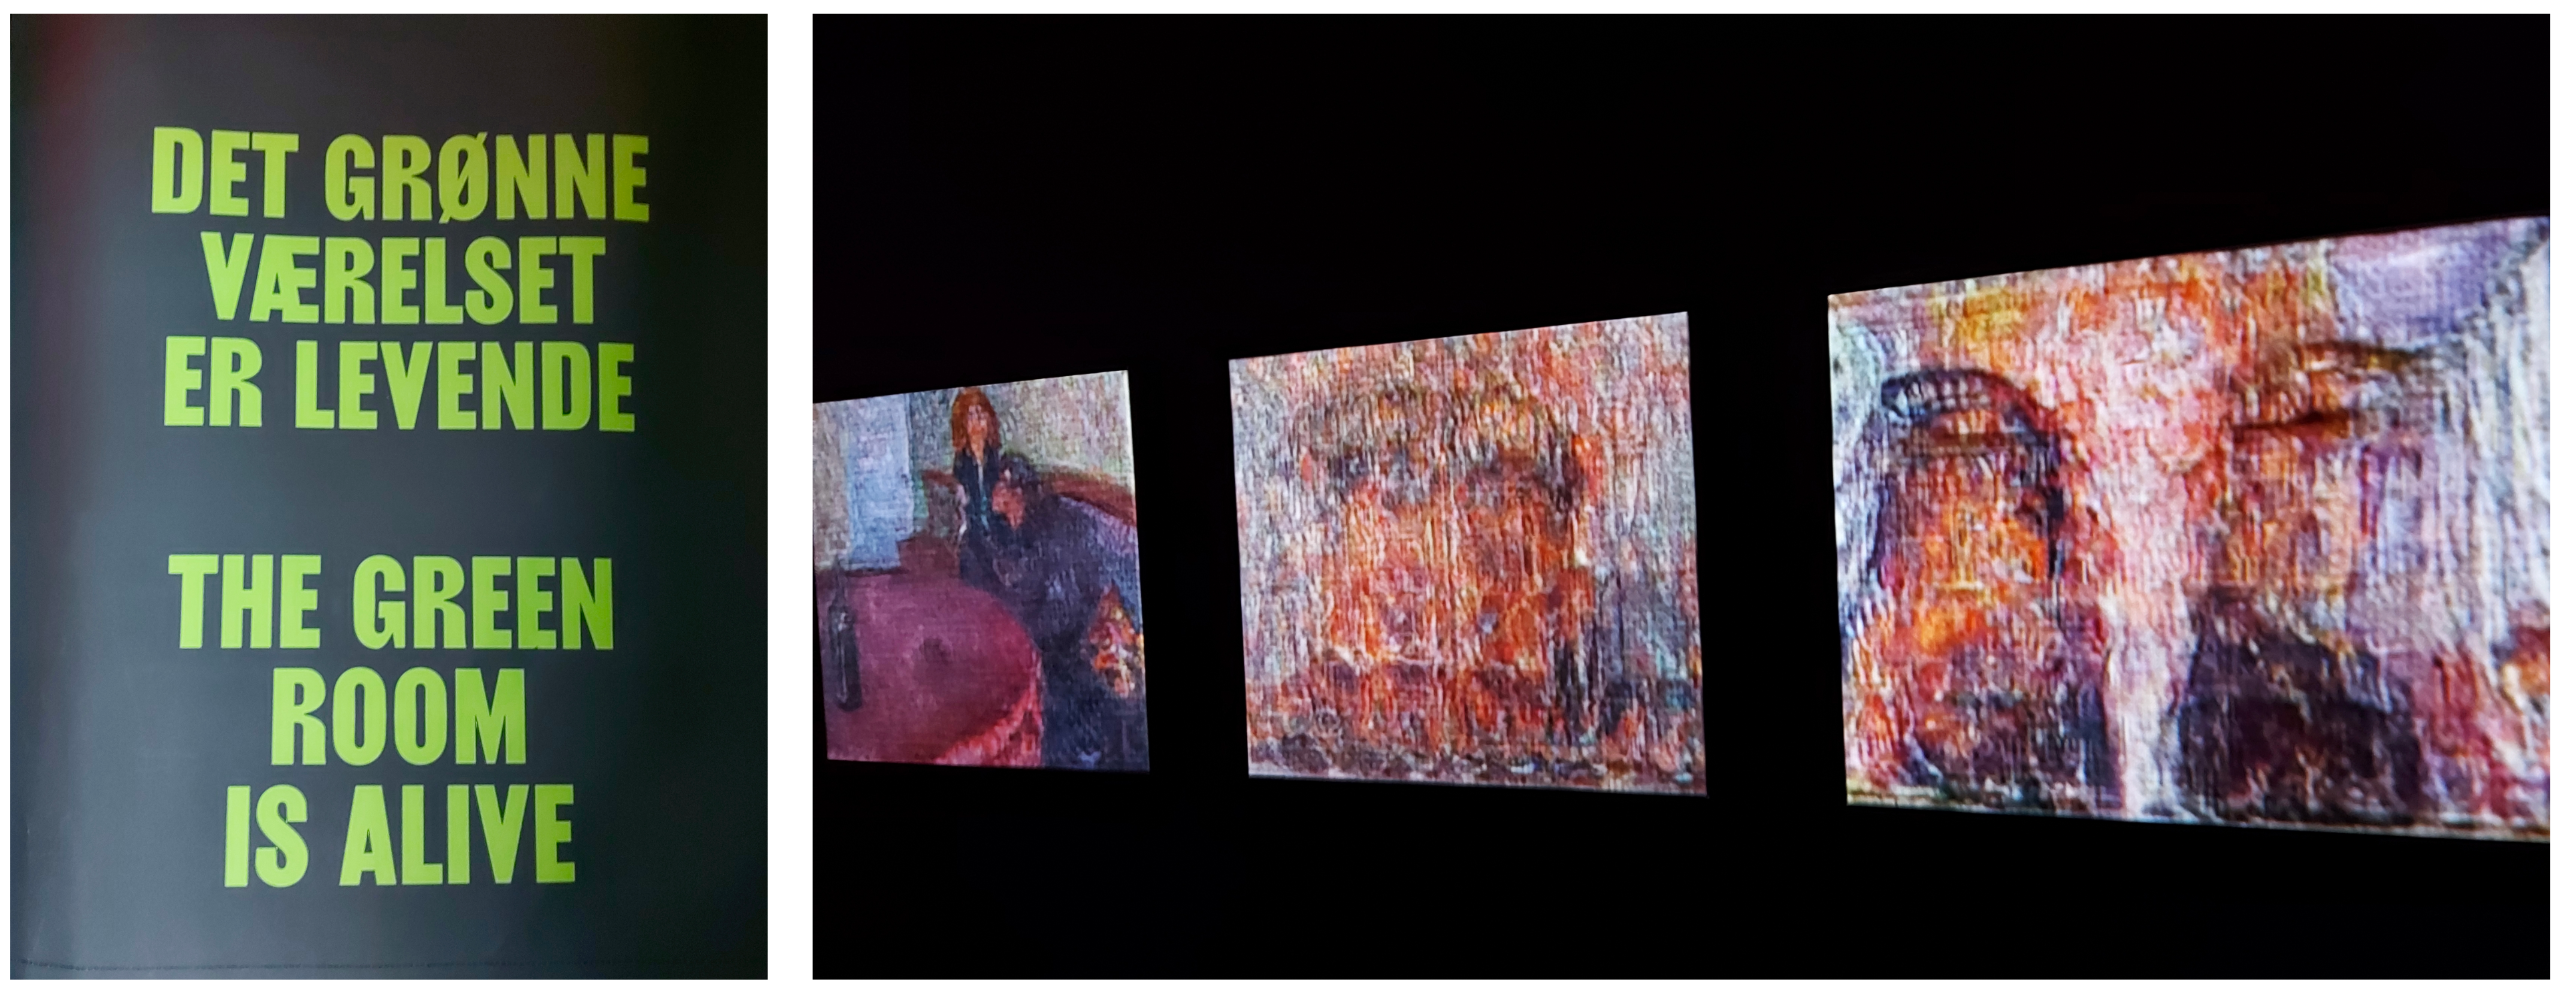
\includegraphics[width=12.5cm]{pictures/process/poison_alive.png}
\caption{Poison: An Edvard Munch Experience}
\centering 
\end{figure}


\section{Shadows by Munch exhibition}
\par
\emph{27.10.2021, excursion to Munch Museum w/ focus on Shadows}
\par

Shadows is one of the permanent exhibitions in the new museum, showcasing Munch's life in the villa Ekely.

This is how the Munch museum describes the exhibition: \emph{"Gain a close understanding of Edvard Munch in a groundbreaking interactive museum experience.
Edvard Munch spent the last 30 years of his life at Ekely, his villa just outside Oslo. The house was demolished in 1960, but in this exhibition we reconstruct Munch’s home in a multimedia installation that uses light, sound and moving images to tell stories from Munch’s life. (...). Join us on a sensory journey back in time that will increase your understanding of Edvard Munch as a person and your knowledge of his surroundings in a biographical exhibition that is unparalleled in the museum world."}


\begin{figure}[H]
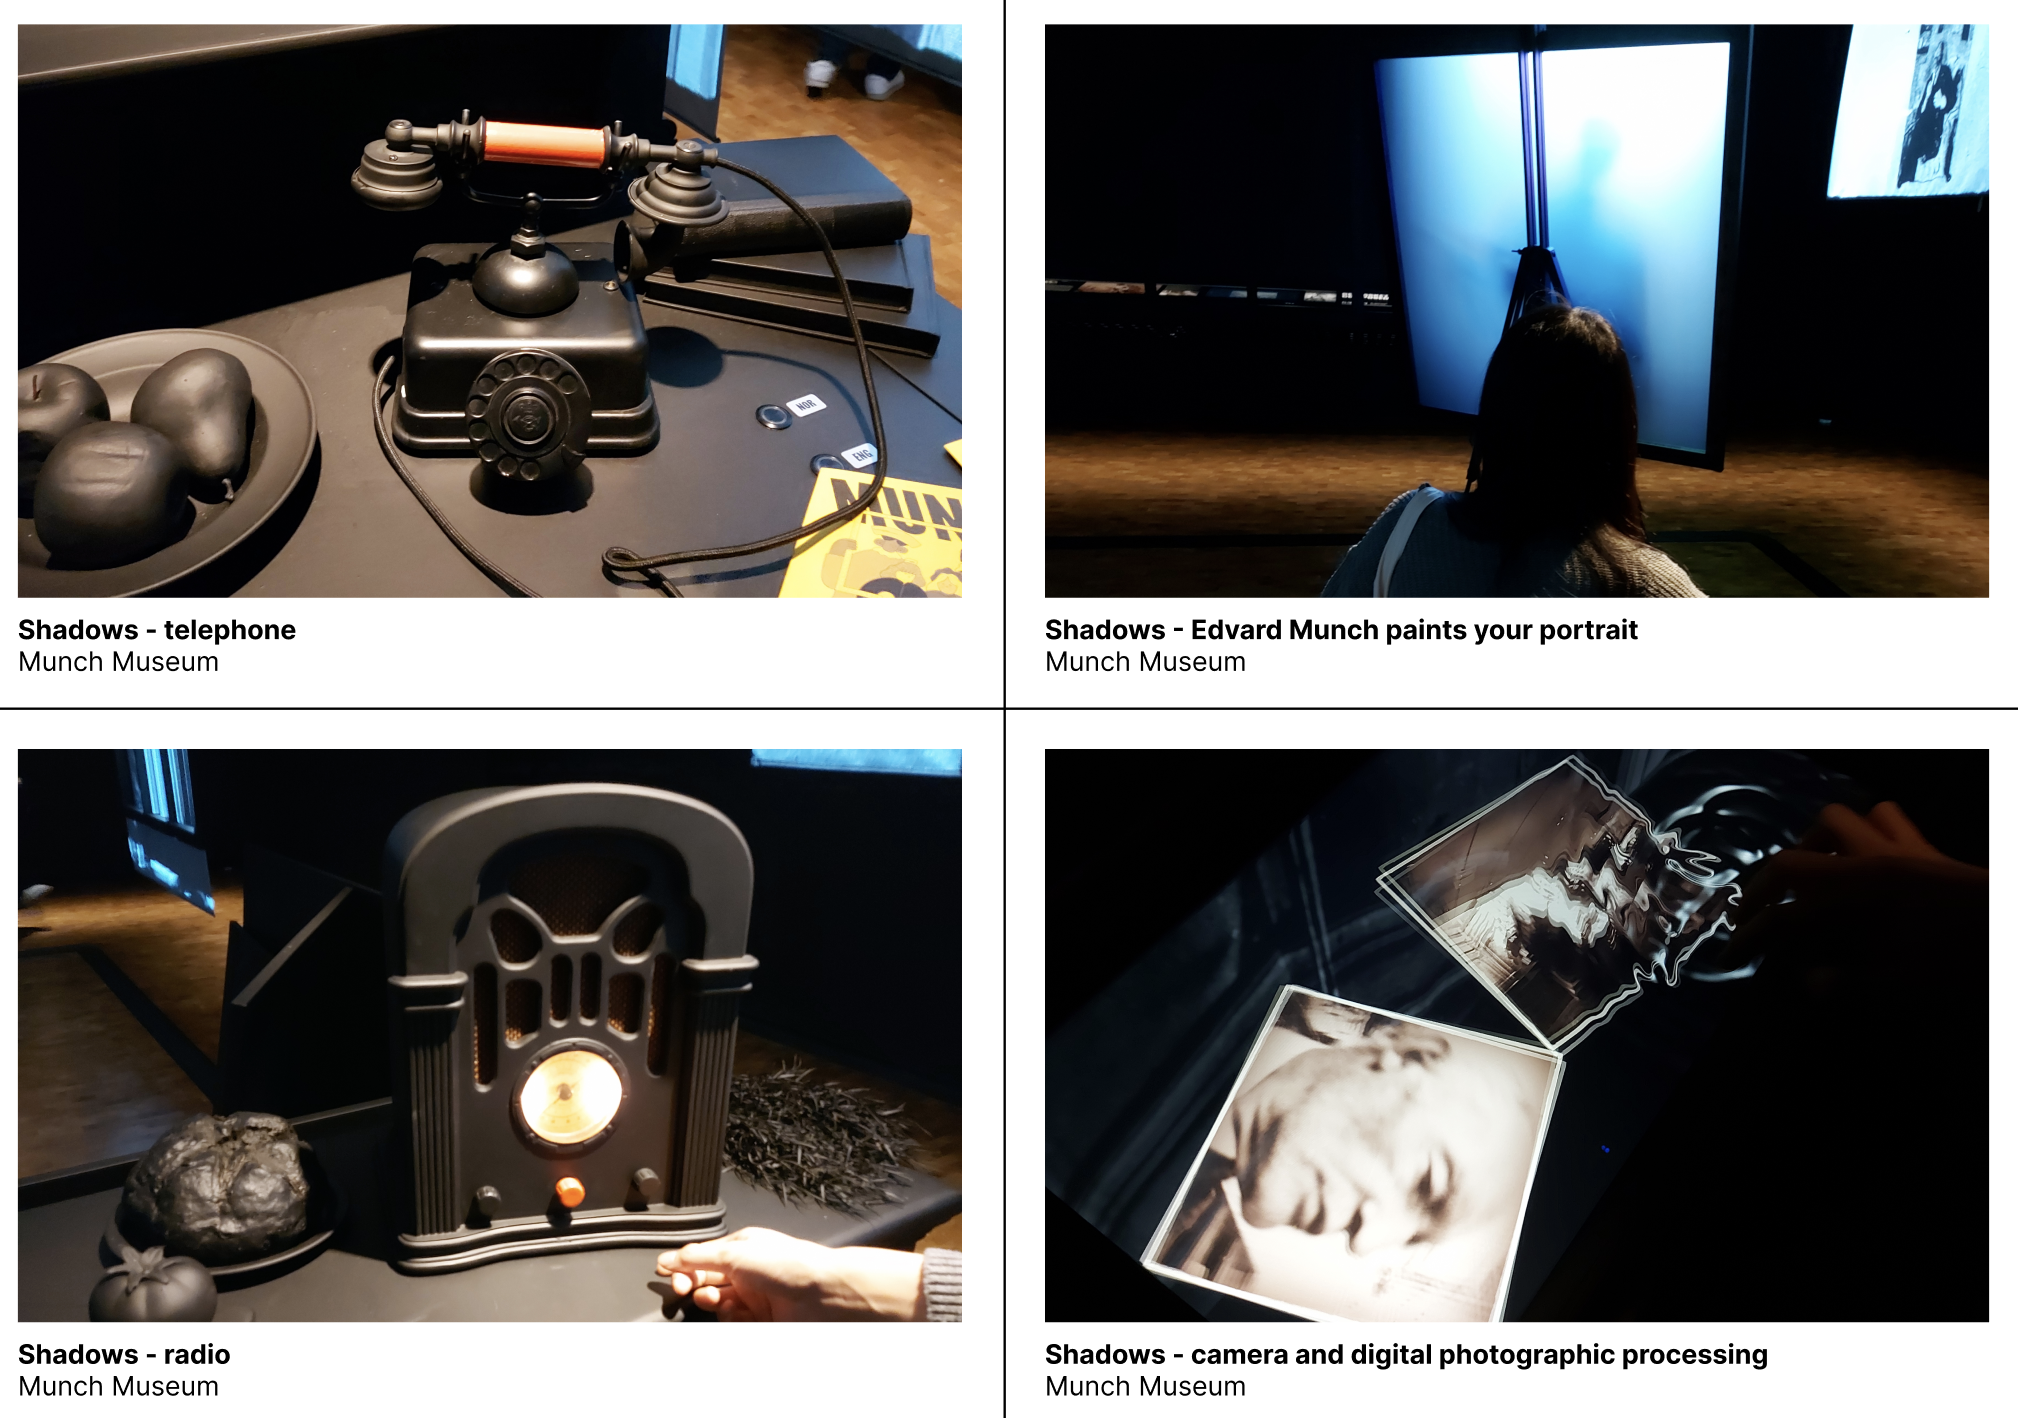
\includegraphics[width=12cm]{pictures/dataset/munch_1.png}
\centering 
\end{figure}


\section{Qi: Energy visualisation workshop}
\emph{09.11.2021, invited to host an energy-visualisation workshop}
\begin{figure}[H]
\includegraphics[width=11cm]{pictures/dataset/Qi.pdf}
\centering 
\end{figure}

In one of the days following/after the slow design exhibition, my design group was contacted by a professor whose field of research lies in the intersection between technology and society, especially concerned with sustainability. She supervises master-students, and for the upcoming year she is supervising thesises concerned with energy visualisations in the new life-sciences building.  



\section{Observing Klimahusets narrative storytelling in-action}
\par
\emph{Observation and interview 16.02.2022}
\par

After my readings on the museum and its expository agency, I wonder what Klimahuset’s stakeholders thoughts are on their agency? And their position toward whether or not they have a subjective or objective expository agency? What are the cultural attitudes, decisions, views and stances the agents involved in designing the climate exhibition in Klimahuset, took before they decided to do the act of exposing? What cultural function does the objects on display in Klimahuset pose? 

Some of these questions can already kind of be elaborated for, from initial reading on internal documents that I have gotten access through collaborating partners in Klimahuset, as well as from conversations with stakeholders from Klimahuset last semester through the workshop, mail correspondence and mini-exhibition. As accounted for in Klimahusets founding documents, their vision/ purpose of the museum is as follows:
To give the visitors an understanding of the most important climate processes that affect the living conditions on Earth so that they are able to develop their own views on climate change, take part in climate discussions or act in other ways in relation to the topic.
Visitors must gain an understanding that natural conditions also affect social structures and culture.
	
Building on Mieke Bal’s narrative analysis on cultural imperialism in museums, say we look at Klimahuset as an ethnographic museum with the expository agency to display installations, objects and data related to the climate crisis. And with a distinct and clear target group being children aged 10-14. Is Klimahusets agency and vision an attempt to display the climate crisis as a current/ ongoing discourse with the function to educate and stimulate critical reflections on current societal norms and ways of living, or is the agency to define and lay up cultural change, to a more sustainable way of living? Maybe both? If so, then comes the question if the museums cultural stakeholders, with this expository agency, are they cultural moralists? Especially because their whole museum exhibition are designed to engage children aged 10-14, though welcoming all age groups, raises the question if the museum and exhibition design in itself potentially have any moral imperialistic function as well, as to who the discourse (the climate crisis) is relevant for. 
Asked the klimaverter about  this, need to do some structural analysis of some sort….

\begin{figure}[H]
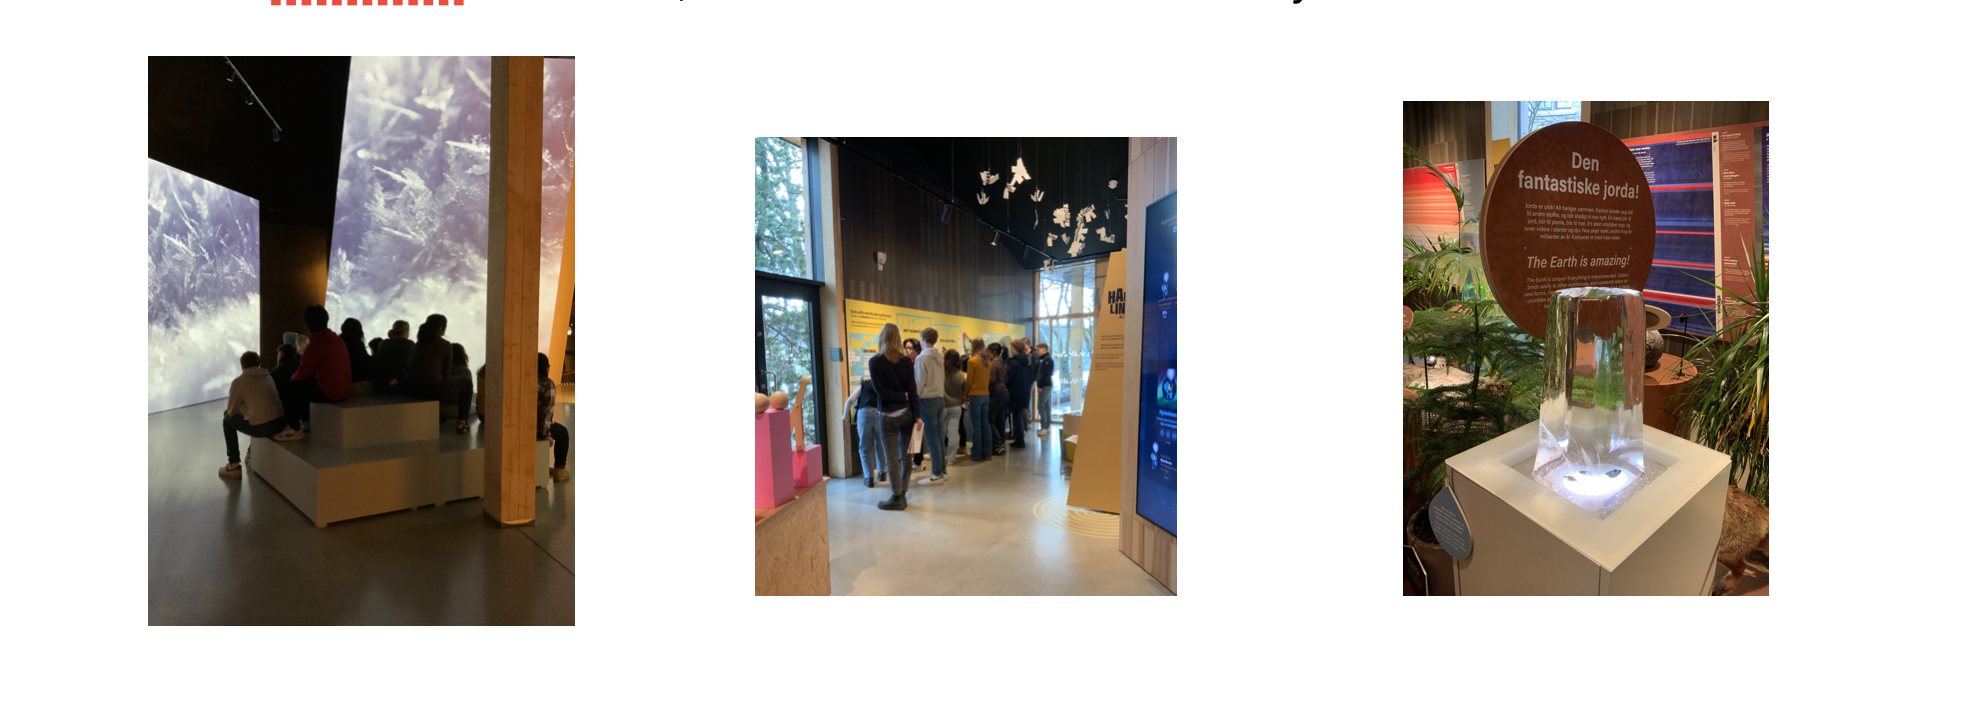
\includegraphics[width=13cm]{pictures/elever_i_klimahuset.png}
\centering 
\end{figure}

Med en klimavert til stede får man bedre hjelp og en form for retning til å “lese” installasjonene, som støtter deg når du senere går gjennom avdeling for avdeling. 
Man blir stilt spørsmål som er knyttet til faktiske ting, som for eksempel i video-atriet sier klimavert; jeg er 160cm høy, hvor høy tror dere denne veggen er?
Etter litt håndsopprekning får vi vite at dersom Grønlandsisen smelter vil havet stige like høyt som det den veggen er. Det er tankevekkende og setter inntrykk!

Her blir man også litt senere spurt: ser dere vær eller klima? et åpent spørsmål som setter i gang en god diskusjon på forskjellen mellom vær og klima, med fokus på hvordan vær påvirker klima. Dette blir forklart at mange blander og tenker at vær og klima er det samme, og at klimaforandringer og værforandringer ikke er det samme. Her får noen elever aha-øyeblikk.


Et annet eksempel er isbiten inne i “den naturlige avdelingen”.  Først får elevene i oppgave å finne noe i området som påvirker klimaet naturlig. Senere når det blir tatt en liten runde spør verten; har alle tatt på isbiten? For så å gå videre til å forklare hvordan menneskelig påvirkning påvirker klimaet. “For eksempel har deres varme hender bidratt til å smelte litt av isbiten her i Klimahuset”. Dette er også tankevekkende og setter inntrykk!


Ice Cube: a good example of a meaningful relation. !!!


\section{Interview with a concept developer from Munch}
\par
\emph{date date date}
\par


\emph{"Det beste er jo når folk lærer noe nytt uten at de merker det, det burde jo være målet og det kan jo være tekst for eksempel som byr på en veldig engasjerende historie men det kan også være noe interaktivt, f.eks. du tar en selfie og at Munch også gjorde det og lagde disse effektene, og kanskje man blir litt interessert i det og kan finne ut mer om det andre steder i museet, som f.eks. i “uendelig utstilling” er det også sånn at vi mener at de forskjellige utstillinger er jo ..(?) av hverandre (at de bygger på hverandre?) og skaper altså verdi for hverandre, at folk som har vært i skygger har muligheten å oppleve Munchs kunst på nye måter ved gå inn i uendelige [avdeling]. Men vi jobber også med nye utstillingsprosjekter der vi, der den tilknytningen mellom digitale opplevelser og mer tradisjonelle presentasjoner av kunst er mer tettere, f.eks. at du at man har sånne immersive rom eller opplevelser i en utstillingssal man kan gå inn i og så ut igjen og oppleve kunsten på en ny måte. Det syns vi er en veldig produktiv måte for å åpne opp utstillingssaler for et større publikum og engasjere flere og bredere. [Her sier B: ja flere perspektiver eller, men tok ikke det på egen linje]. Ja. Vi ser det også med Poison [utstilling] f.eks., mange som likte det hadde også behov for å se originalbildene f.eks. Så det tror jeg er absolutt noe som ikke erstatter originalkunsten, som mange frykter, men må være som beriker og gir deg kanskje en, gir også visse grupper en sjans for at de gidder å befatte seg med det eller se på kunsten og ikke bare, de fleste ser jo bare i 3 eller 5 sekunder på et bilde og så gå videre til neste. Uten formiddling er det ikke noen sjanse for å øke den tiden enkelte tilbringer med kunsten."}

